In this chapter the results from the experiments will be shown and analyzed. First, the model will be discussed without any policies in effect. Following this, the base model is tested for it's performance against multiple scenarios. Finally, the policies are implemented, and their robustness to the earlier scenarios tested. This analysis serves an interpretation of the relative cost-effectiveness of the chosen policies, allowing for comparison of real-world cost of implementation. 

\iffalse
1.	Show and explain results without policies
2.	Show and explain consequences of scenarios for model behaviour
3.	Show and explain consequences of policies for each scenario (i.e., robustness) 
\fi
\subsection{Base Model}

The model was first run without any policies in place to study the effects of the scenarios on the situation as is. Afterwards, it will be run as a part of the scenarios to see how the status quo fares in our defined scenarios. 

The model was run without any scenarios to generate behaviour, dubbed the base run. The behaviour of the KPIs was studied for this base behaviour.

\begin{figure}[h!]
    \centering
    \begin{minipage}{0.45\textwidth}
        \centering
        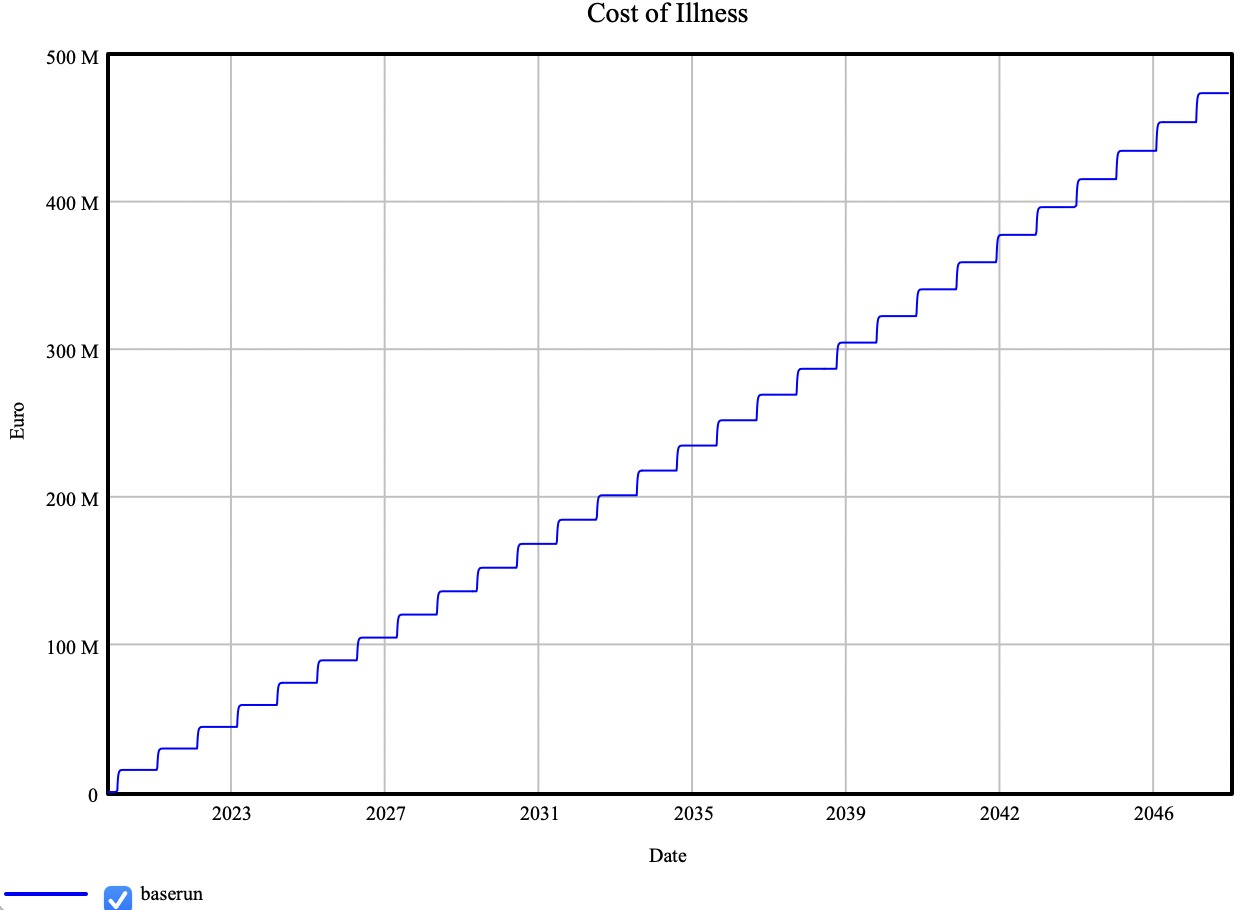
\includegraphics[width=1\textwidth]{images/base_COI.jpeg} % first figure itself
        \caption{Cost of Illness in the base run}
        \label{fig:b_coi}
    \end{minipage}\hfill
    \begin{minipage}{0.45\textwidth}
        \centering
        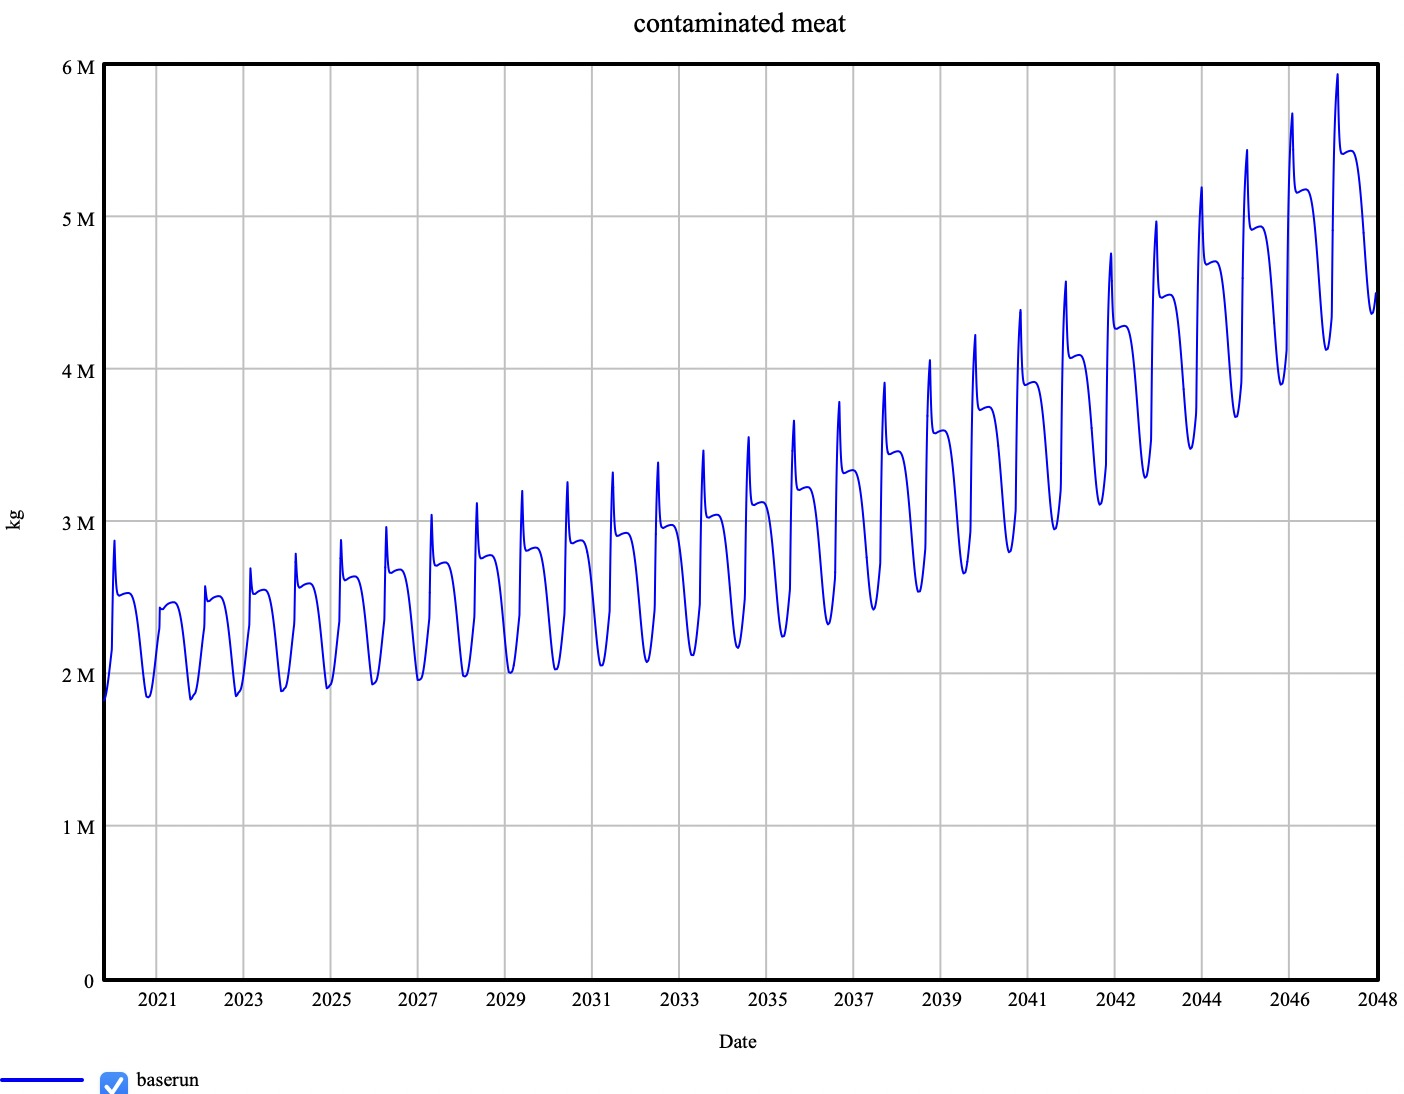
\includegraphics[width=1\textwidth]{images/base_meat.jpeg} % second figure itself
        \caption{Contaminated chicken meat in the base run}
        \label{fig:b_meat}
    \end{minipage}
\end{figure}

\begin{figure}[h!]
    \centering
    \begin{minipage}{0.45\textwidth}
        \centering
        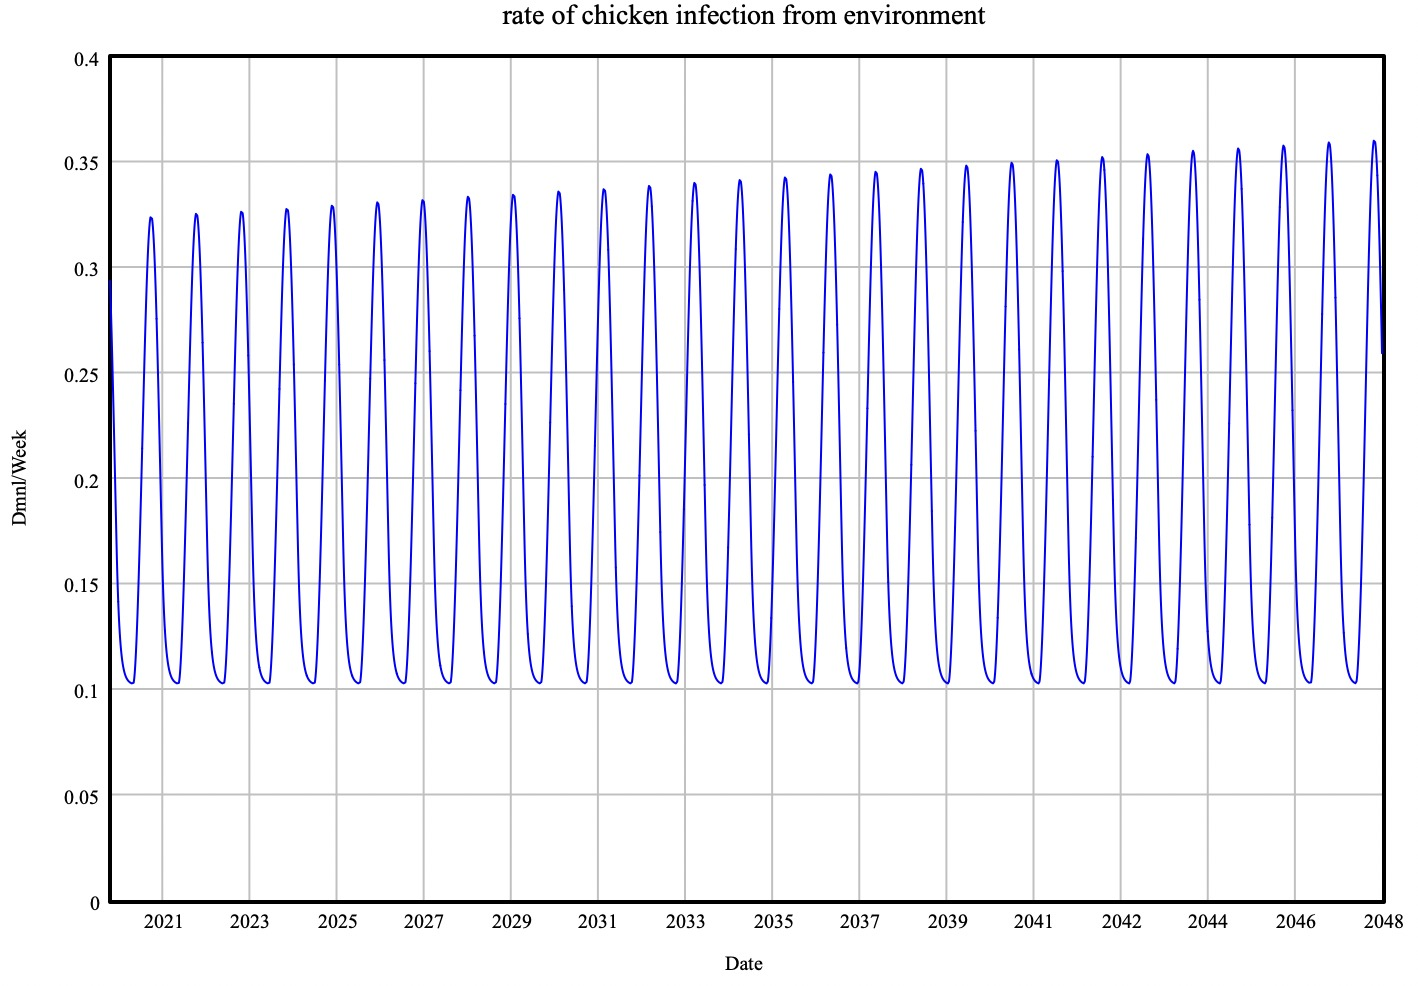
\includegraphics[width=1\textwidth]{images/base_chicken.jpeg} 
        \caption{Chicken infections from environment in the base run}
        \label{fig:b_chicken}
    \end{minipage}\hfill
    \begin{minipage}{0.45\textwidth}
        \centering
        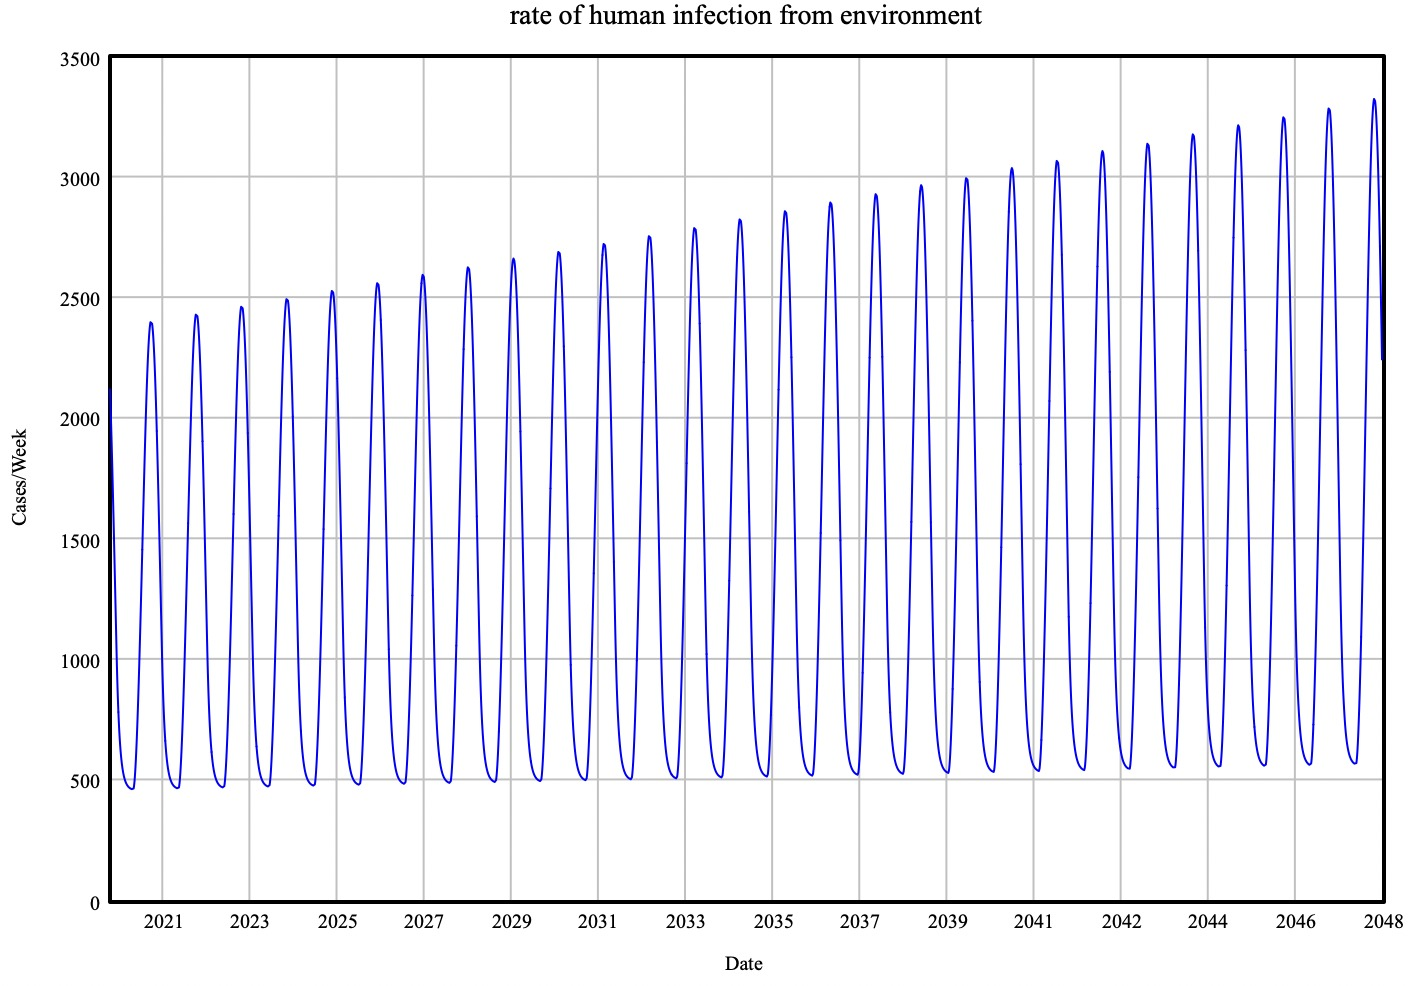
\includegraphics[width=1\textwidth]{images/base_human.jpeg}
        \caption{Human infections from environment in the base run}
        \label{fig:b_human}
    \end{minipage}
\end{figure}

The model generated behaviour that was generally consistent with the dynamic hypothesis, with three main exceptions:

The contaminated meat stock (Figure \ref{fig:b_meat}) exhibits unusual behaviour due to a structural uncertainty linking the number of \textit{campylobacter} cases to changes in meat consumption. After a given threshold number of cases have occurred in the population, we assume there would be a change in behaviour of people choosing to consume less chicken meat to avoid infections, this results in a temporary spike in the contaminated meat stock while the poultry industry responds to changing consumer demand.

Secondly, we did not account for seasonality in the development of the contaminated meat stock. It had been conceptualised in the aggregate sense, leaving the seasonality out of it. 

The model produces a stair-like graph for the cost of illness, where we had hypothesized a straight line instead. This has to with the switch in units mentioned in section \ref{s:verification}, where the model goes from weeks to years. This means that the increase in Cost of Illness occurs once every 52 weeks and then remains the same for the rest of the year, resulting in the stairs we can see in (Figure \ref{fig:b_coi}). Should the time step of the model have been consistent, it would have resulted in a straight line as hypothesized. 


\subsection{Policy Robustness}
In this section, results of scenario testing of each of the policies was examined, to understand which policies were most robust and most cost effective, to inform policy recommendations.

\subsubsection{Safe Slaughtering}
\label{sec: safe slaughtering}
Scenario analysis demonstrated that while safe slaughtering is relatively robust over most scenarios, however it is not generally cost-effective. This is because the policy is addressing infection rates after some number of the flock is already infected, making it more reactive than other policies, which focus on addressing environmental effects.

\begin{figure}[h!]
    \centering
    \begin{minipage}{0.45\textwidth}
        \centering
        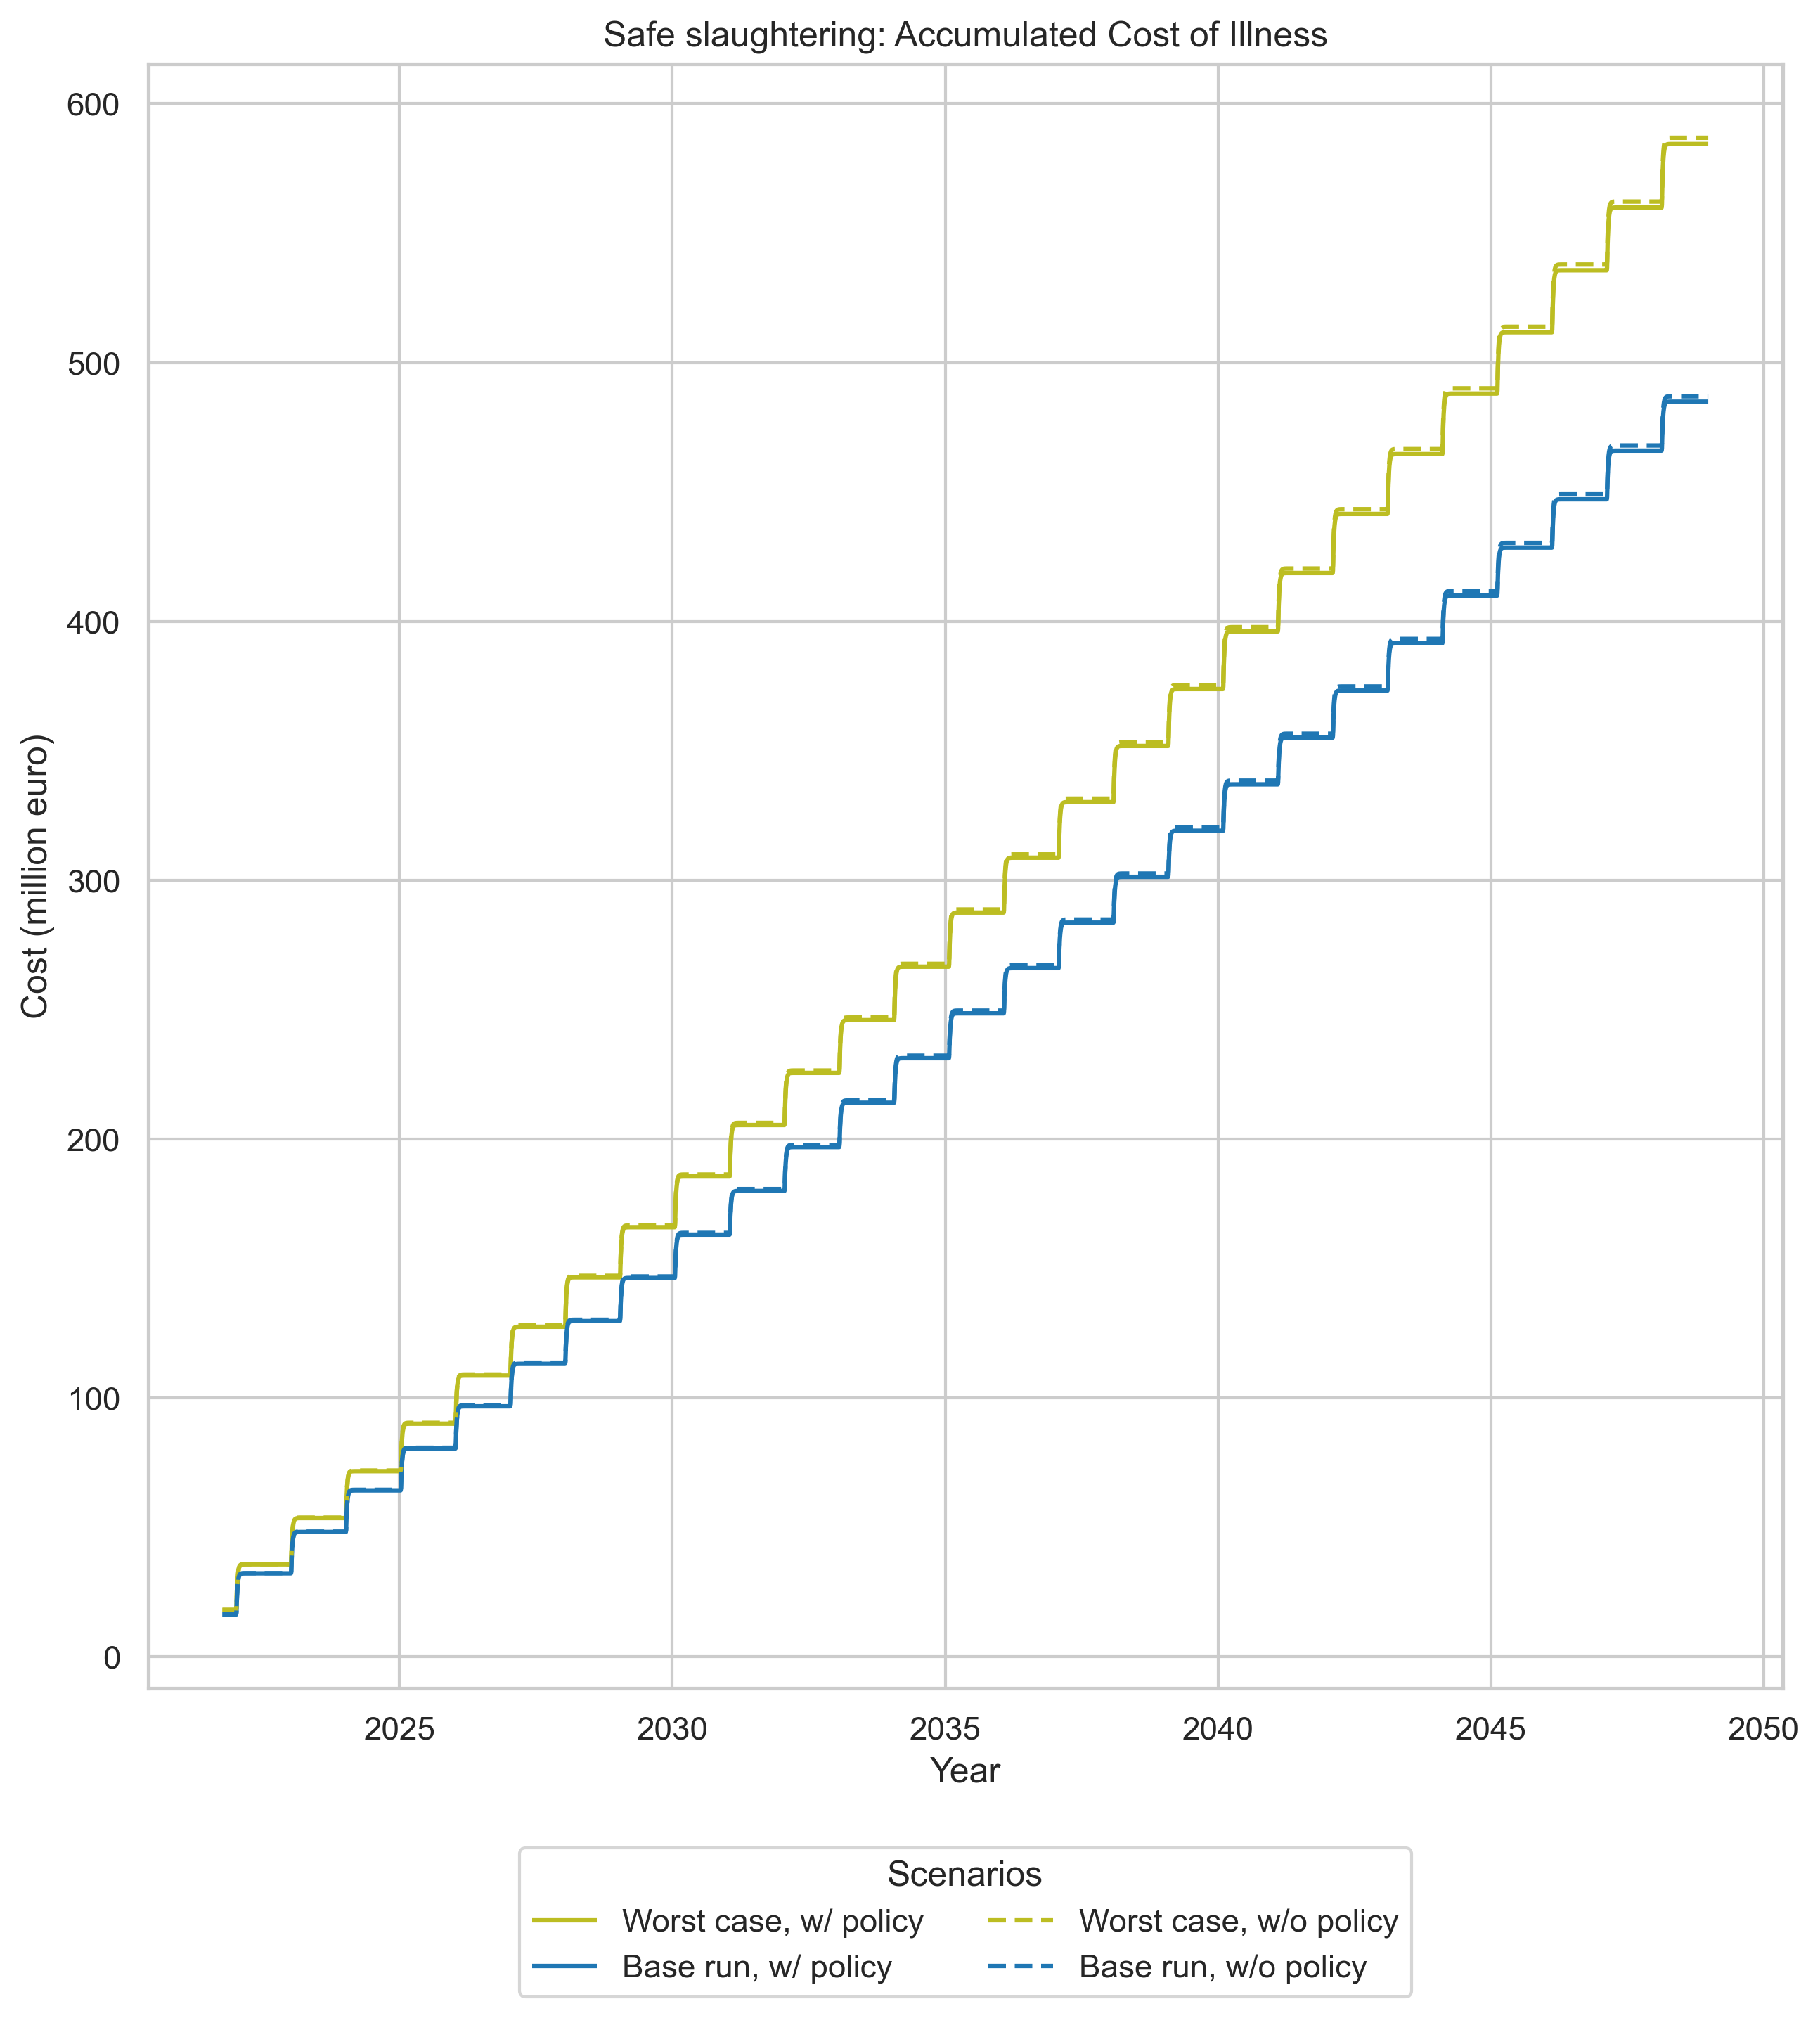
\includegraphics[width=1\textwidth]{images/ss_Base and Worst Case_acoi.png}
        \caption{Accumulated cost of illness under best and worst case scenario, solid lines represent conditions with policy, dashed lines are condition without policy}
        \label{fig:ss_bwc_acoi}
    \end{minipage}\hfill
    \begin{minipage}{0.45\textwidth}
        \centering
        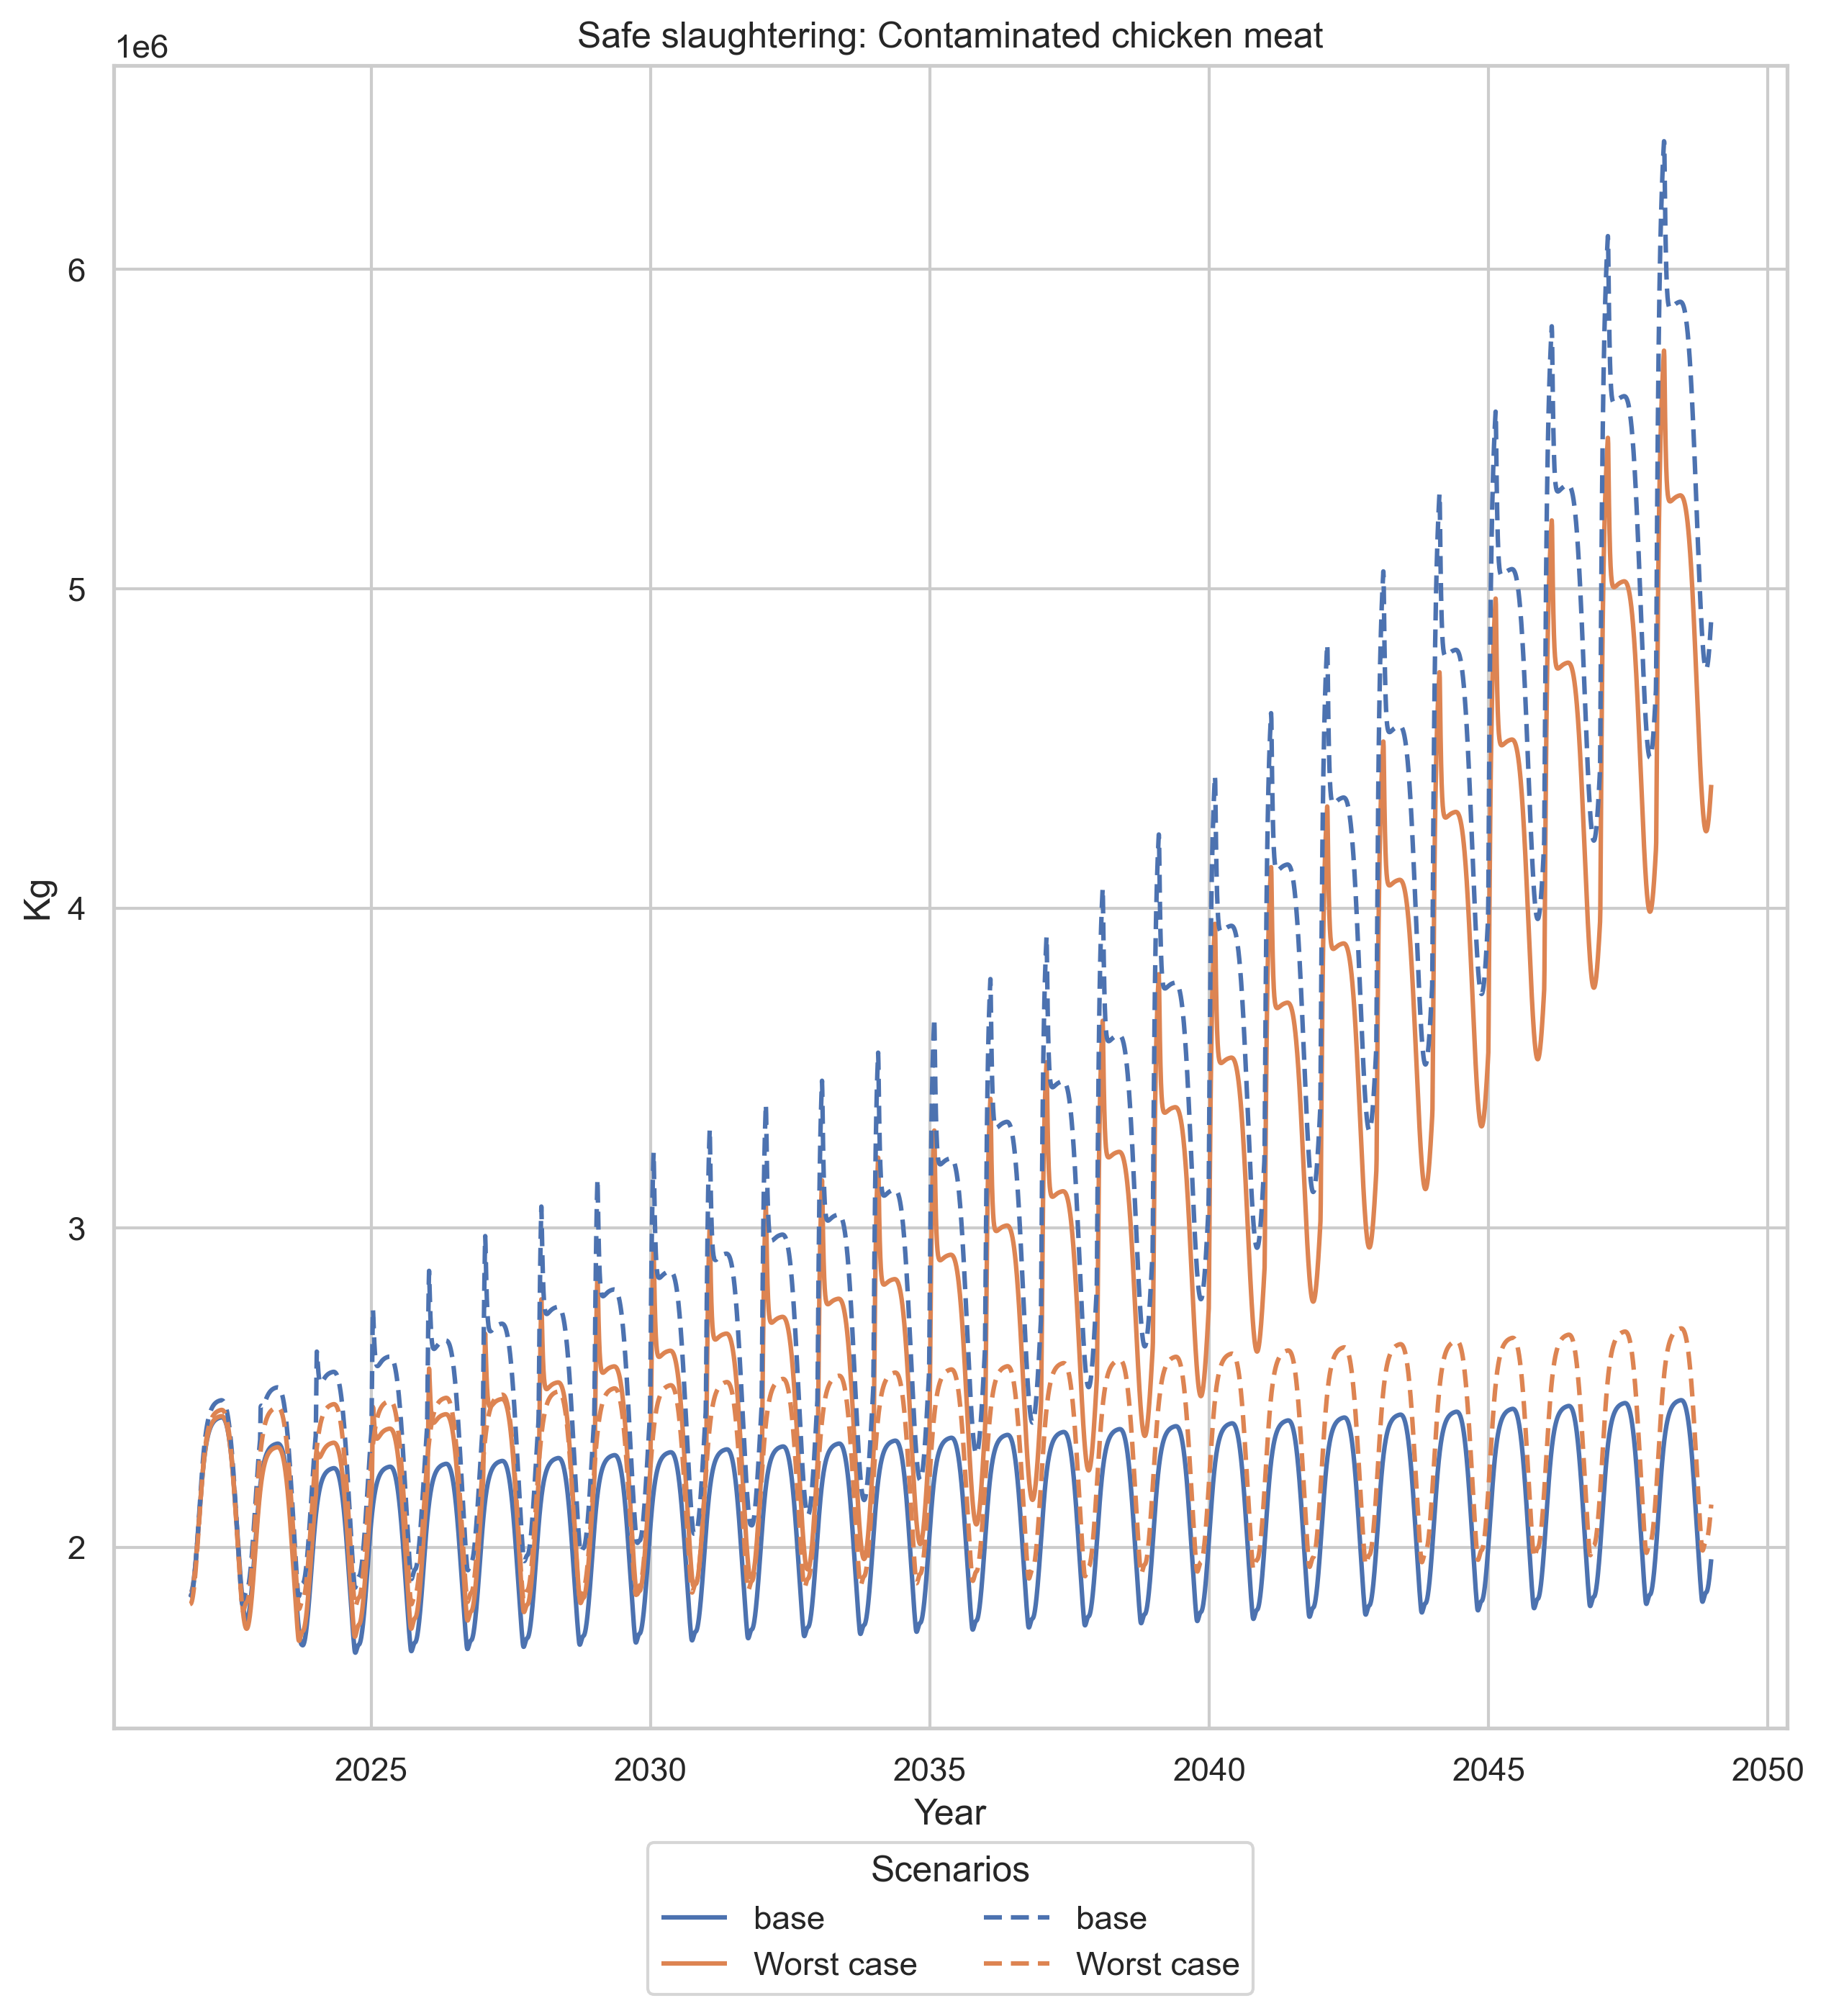
\includegraphics[width=1\textwidth]{images/ss_Base and Worst Case_meat.png} 
        \caption{Contaminated chicken meat in the best and worst case scenario, solid lines represent conditions with policy, dashed lines are condition without policy}
        \label{fig:ss_bwc_meat}
    \end{minipage}
\end{figure}


Interpretation of the cost of illness results across all scenarios demonstrated that only modest economic savings are achieved by implementing a safe slaughtering policy (in the order of ~€0.5 million over the entire thirty year time horizon), as seen in Figure \ref{fig:ss_bwc_acoi}. Further to this, our model doesn't take into account costs to farmers of implementing such a policy, so the aggregate cost effect is unlikely to be positive.

Based on these results, we would not recommend prioritising a safe slaughtering policy over other policies due to it's limited effectiveness. The limited effectiveness is shown explicitly in Figure \ref{fig:ss_bwc_meat}, for intuitively this policy would affect infected chicken meat the most, however, it can be seen that its influence doesn't prevent worst case scenario from occurring. 

\subsubsection{Pest Control}
\label{sec: pest control}
The Pest Control policy was found to be robust against climate change scenarios, with no observable difference between KPI outcomes for different climate scenarios, as can be seen in Figure \ref{fig:pc_seas_meat}. This is because the policy is pegged to temperature, effectively capping propagation of flies at higher temperatures. However, it is less robust to changes in seasonality, wherein after 2030, there is a divergence in outcomes. For scenarios with greater seasonality, the policy of controlling fly populations is less capable of responding to larger variation in temperature. 

\begin{figure}[h!]
    \centering
    \begin{minipage}{0.45\textwidth}
        \centering
        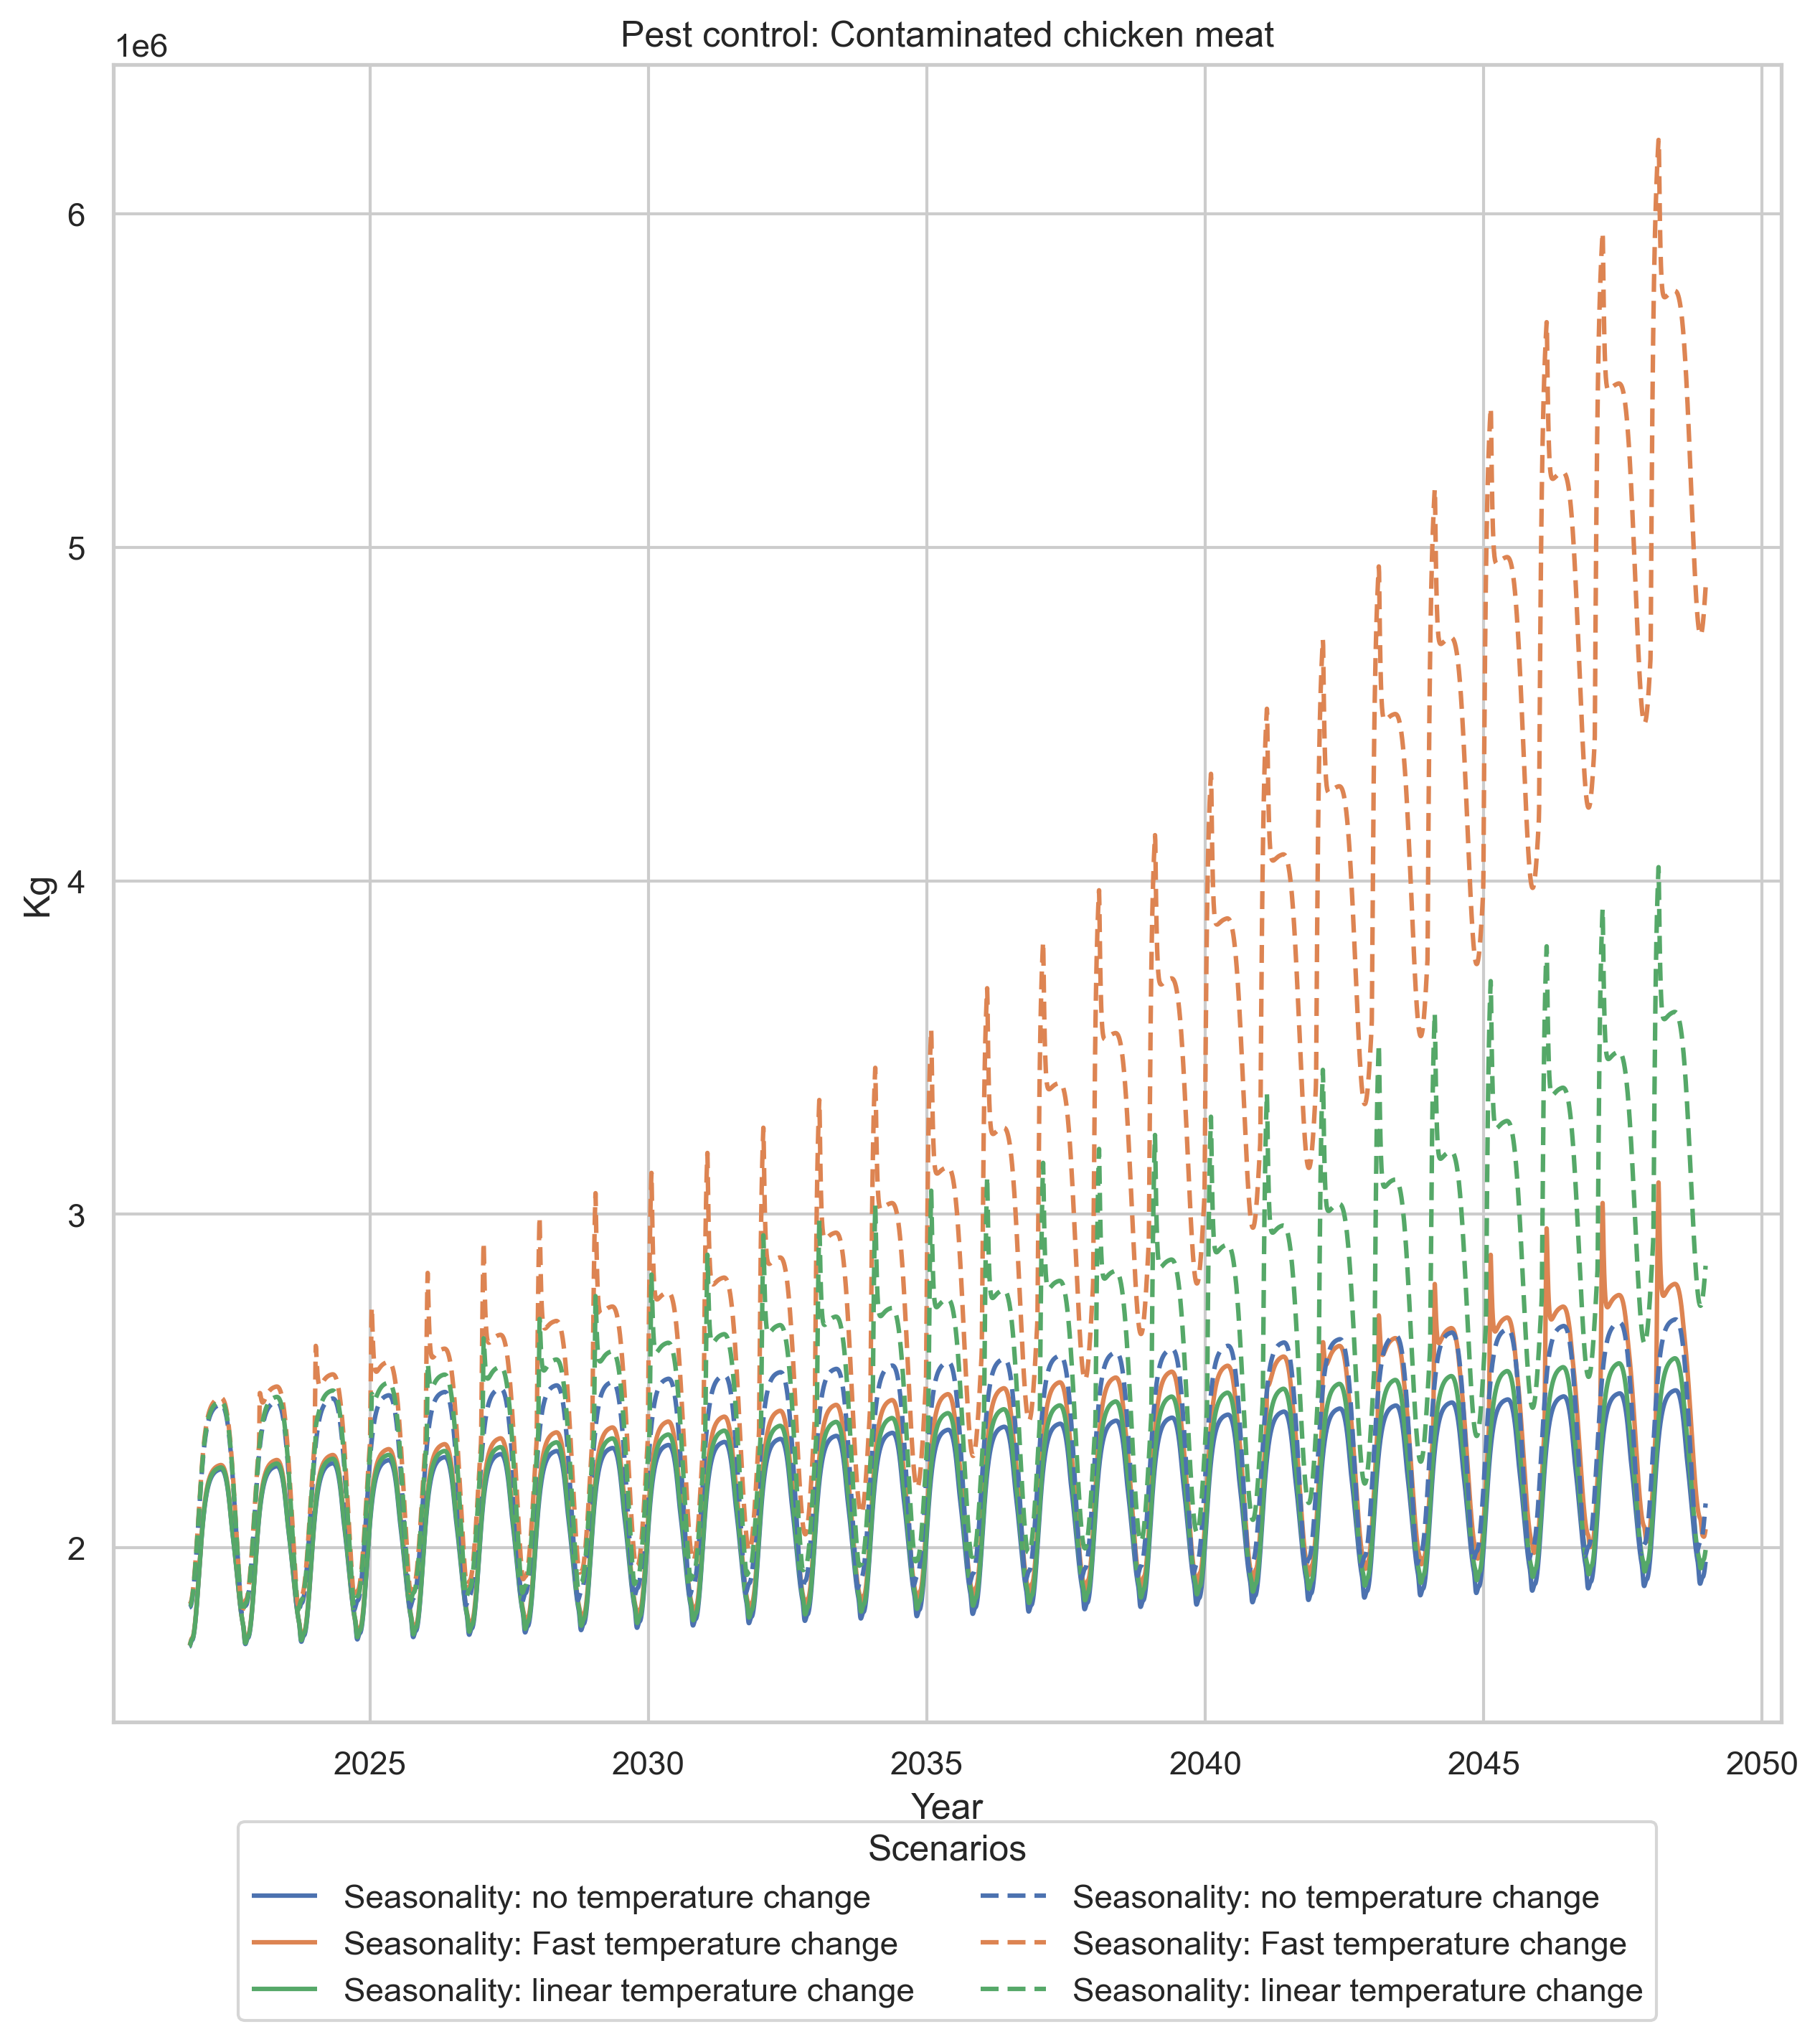
\includegraphics[width=1\textwidth]{images/pc_Seasonal_meat.png}
        \caption{Contaminated chicken meat under different seasonality conditions, solid lines represent conditions with policy, dashed lines are condition without policy}
        \label{fig:pc_seas_meat}
    \end{minipage}\hfill
    \begin{minipage}{0.45\textwidth}
        \centering
        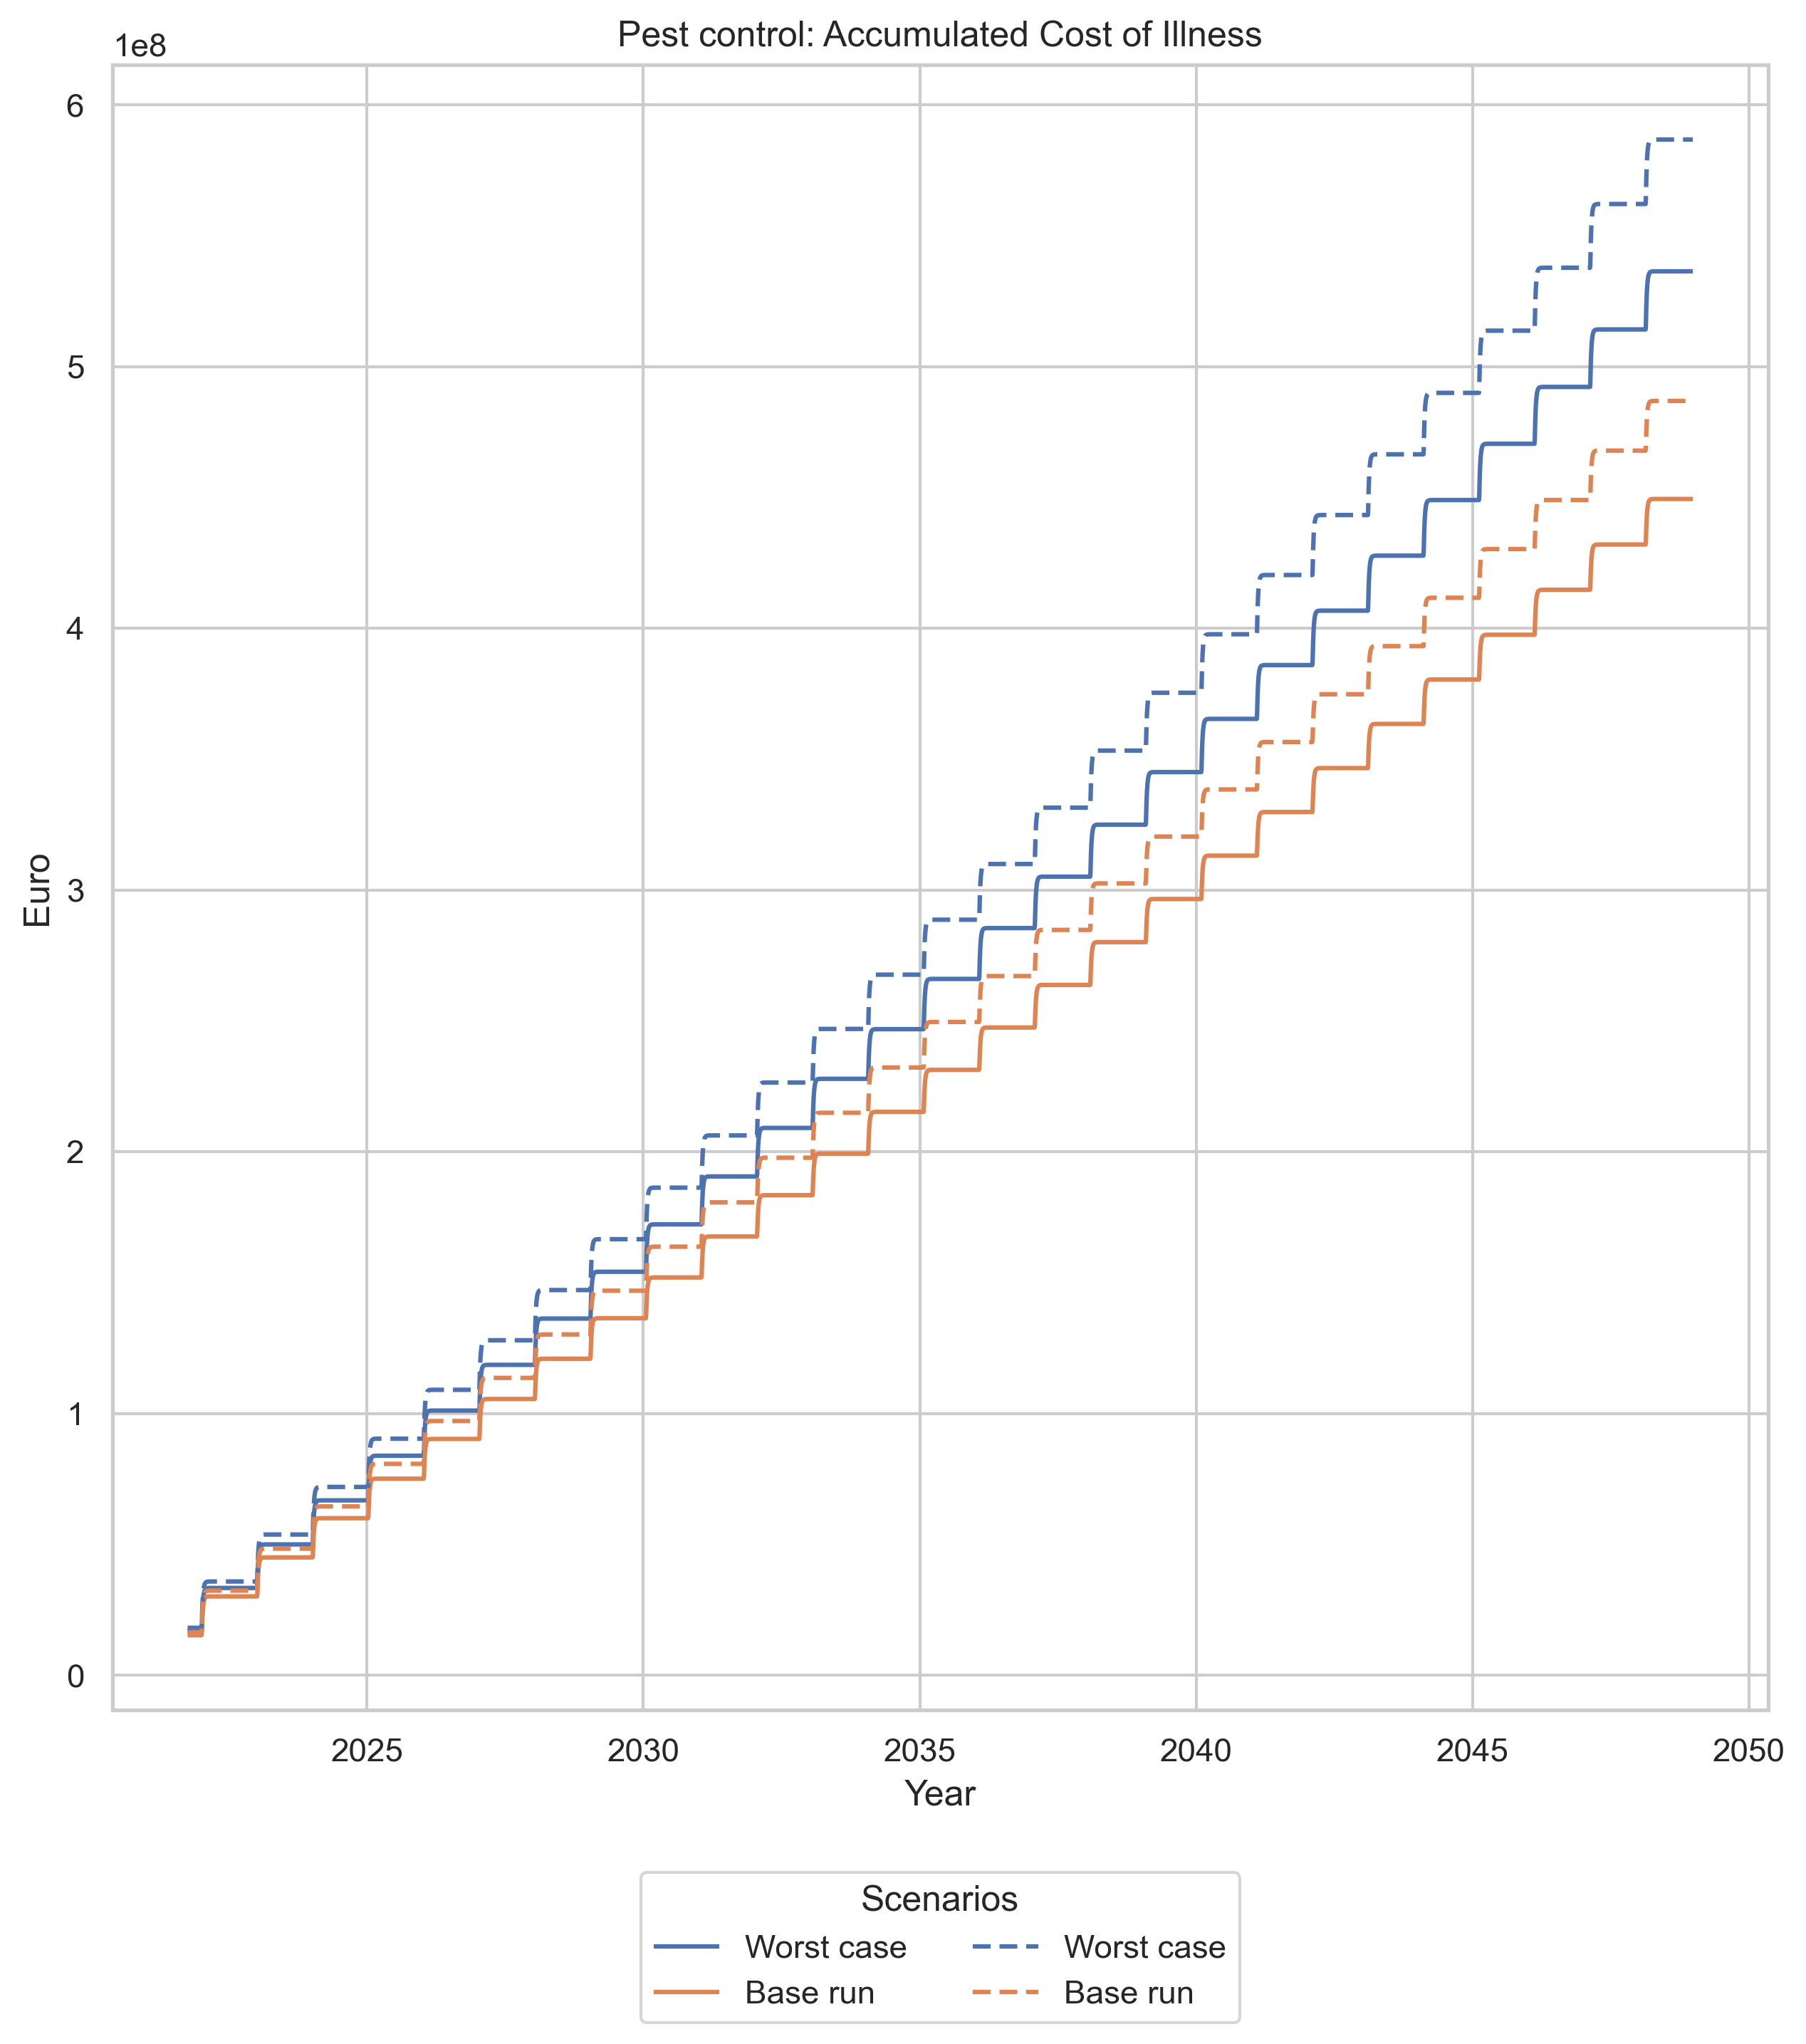
\includegraphics[width=1\textwidth]{images/pc_Base and Worst Case_acoi.png} 
        \caption{Accumulative cost of illness under the base and worst case scenarios, solid lines represent conditions with policy, dashed lines are condition without policy}
        \label{fig:pc_bwc_acoi}
    \end{minipage}
\end{figure}

Predictably, the policy doesn't influence changes in public health scenarios, as the effects are too far downstream of the policy for pest control to have a material impact. 

As pest control is robust to climate variation, we recommend that policy-makers consider this as an effective policy under futures with climate uncertainty, but should be paired with other policies to manage for downstream effects (especially with respect to public health scenarios). In the near term, this policy is unlikely to be cost-effective, however, from 2030 onward (assuming climate projections are representative), the economic effects of the policy will be large enough (more than €10 million) to justify expenditure on this policy, as shown in Figure \ref{fig:pc_bwc_acoi}. 

Note: This policy is implemented without delay. It was assumed that if a policy is in place to exterminate flies once temperature exceeds 20 degrees Celsius, government can effectively trigger an immediate extermination at relevant locations.

\subsubsection{Food safety and handling}
\label{sec: food safety}
The Food Safety policy is a robust policy in terms of reducing food-borne \textit{Campylobacter} infections. This is evidenced in the Figure \ref{fig:fs_pop_meat}
whereby the gap between the amount of contaminated meat with and without the policy in place widens over time across all scenarios. Even under higher population estimates, this policy is effective for reducing this case load.

\begin{figure}[h!]
    \centering
    \begin{minipage}{0.45\textwidth}
        \centering
        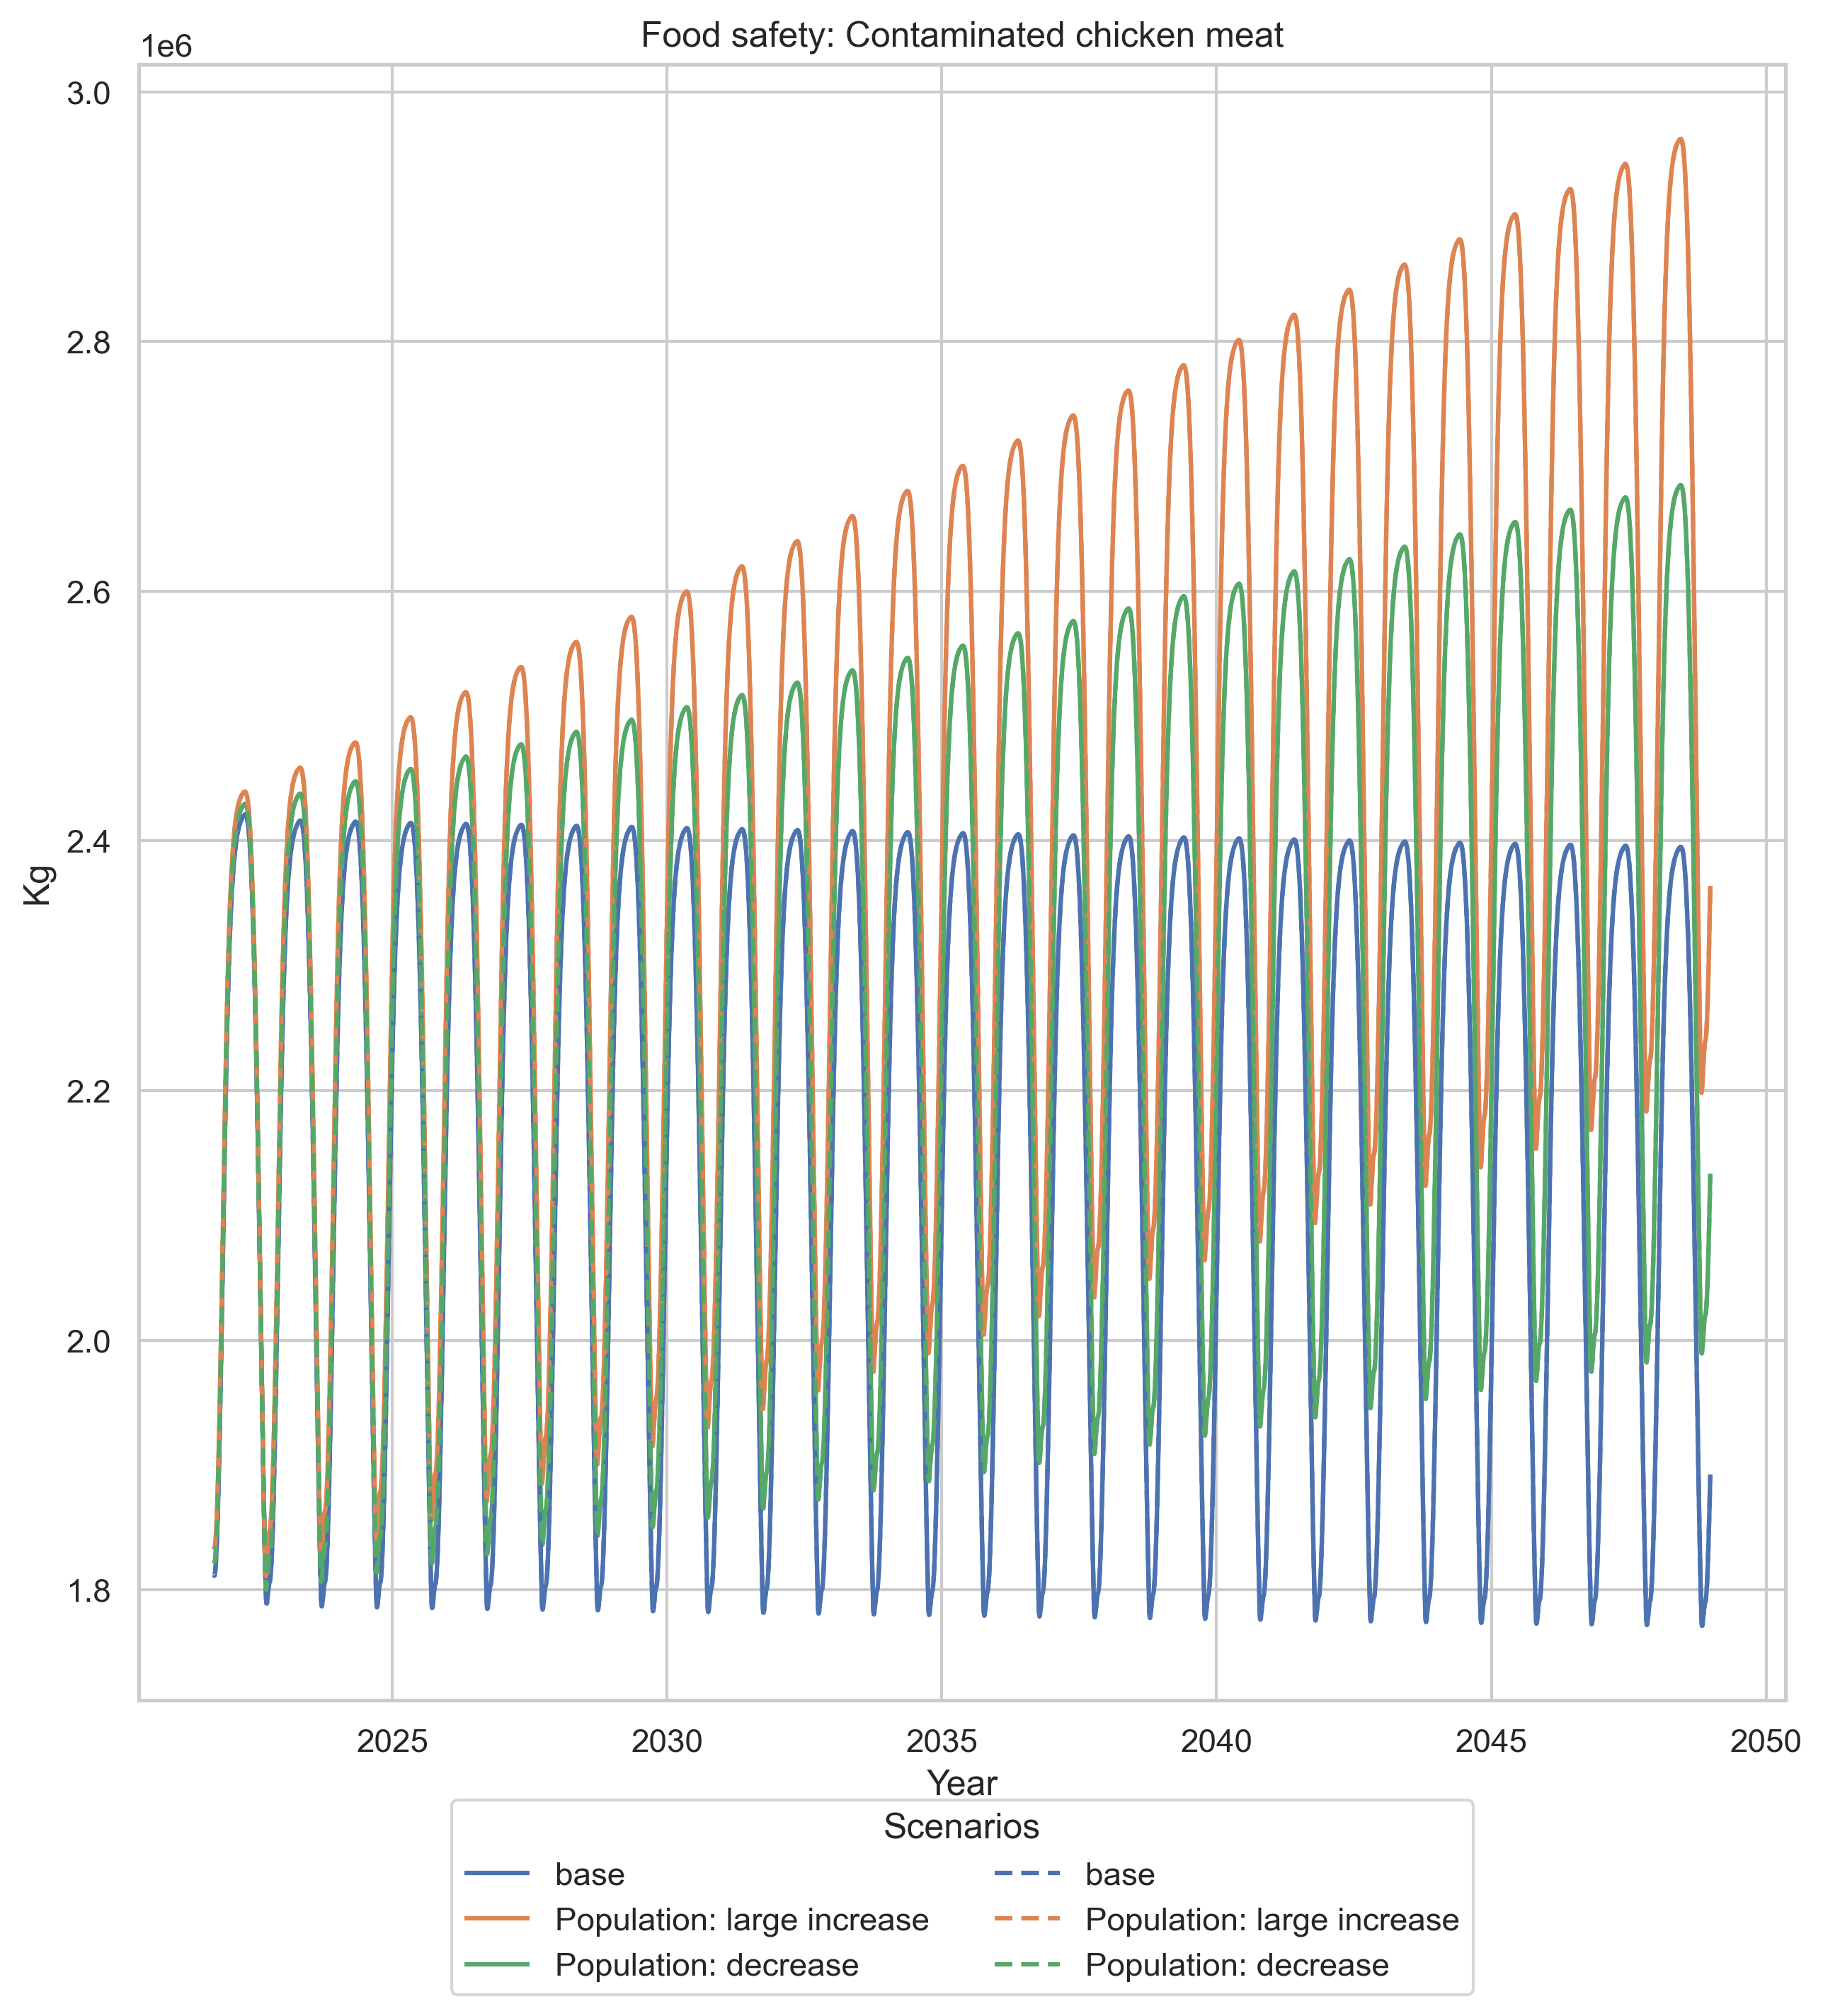
\includegraphics[width=1\textwidth]{images/fs_Population_meat.png}
        \caption{Contaminated chicken meat under different population scenarios, solid lines represent conditions with policy, dashed lines are condition without policy}
        \label{fig:fs_pop_meat}
    \end{minipage}\hfill
    \begin{minipage}{0.45\textwidth}
        \centering
        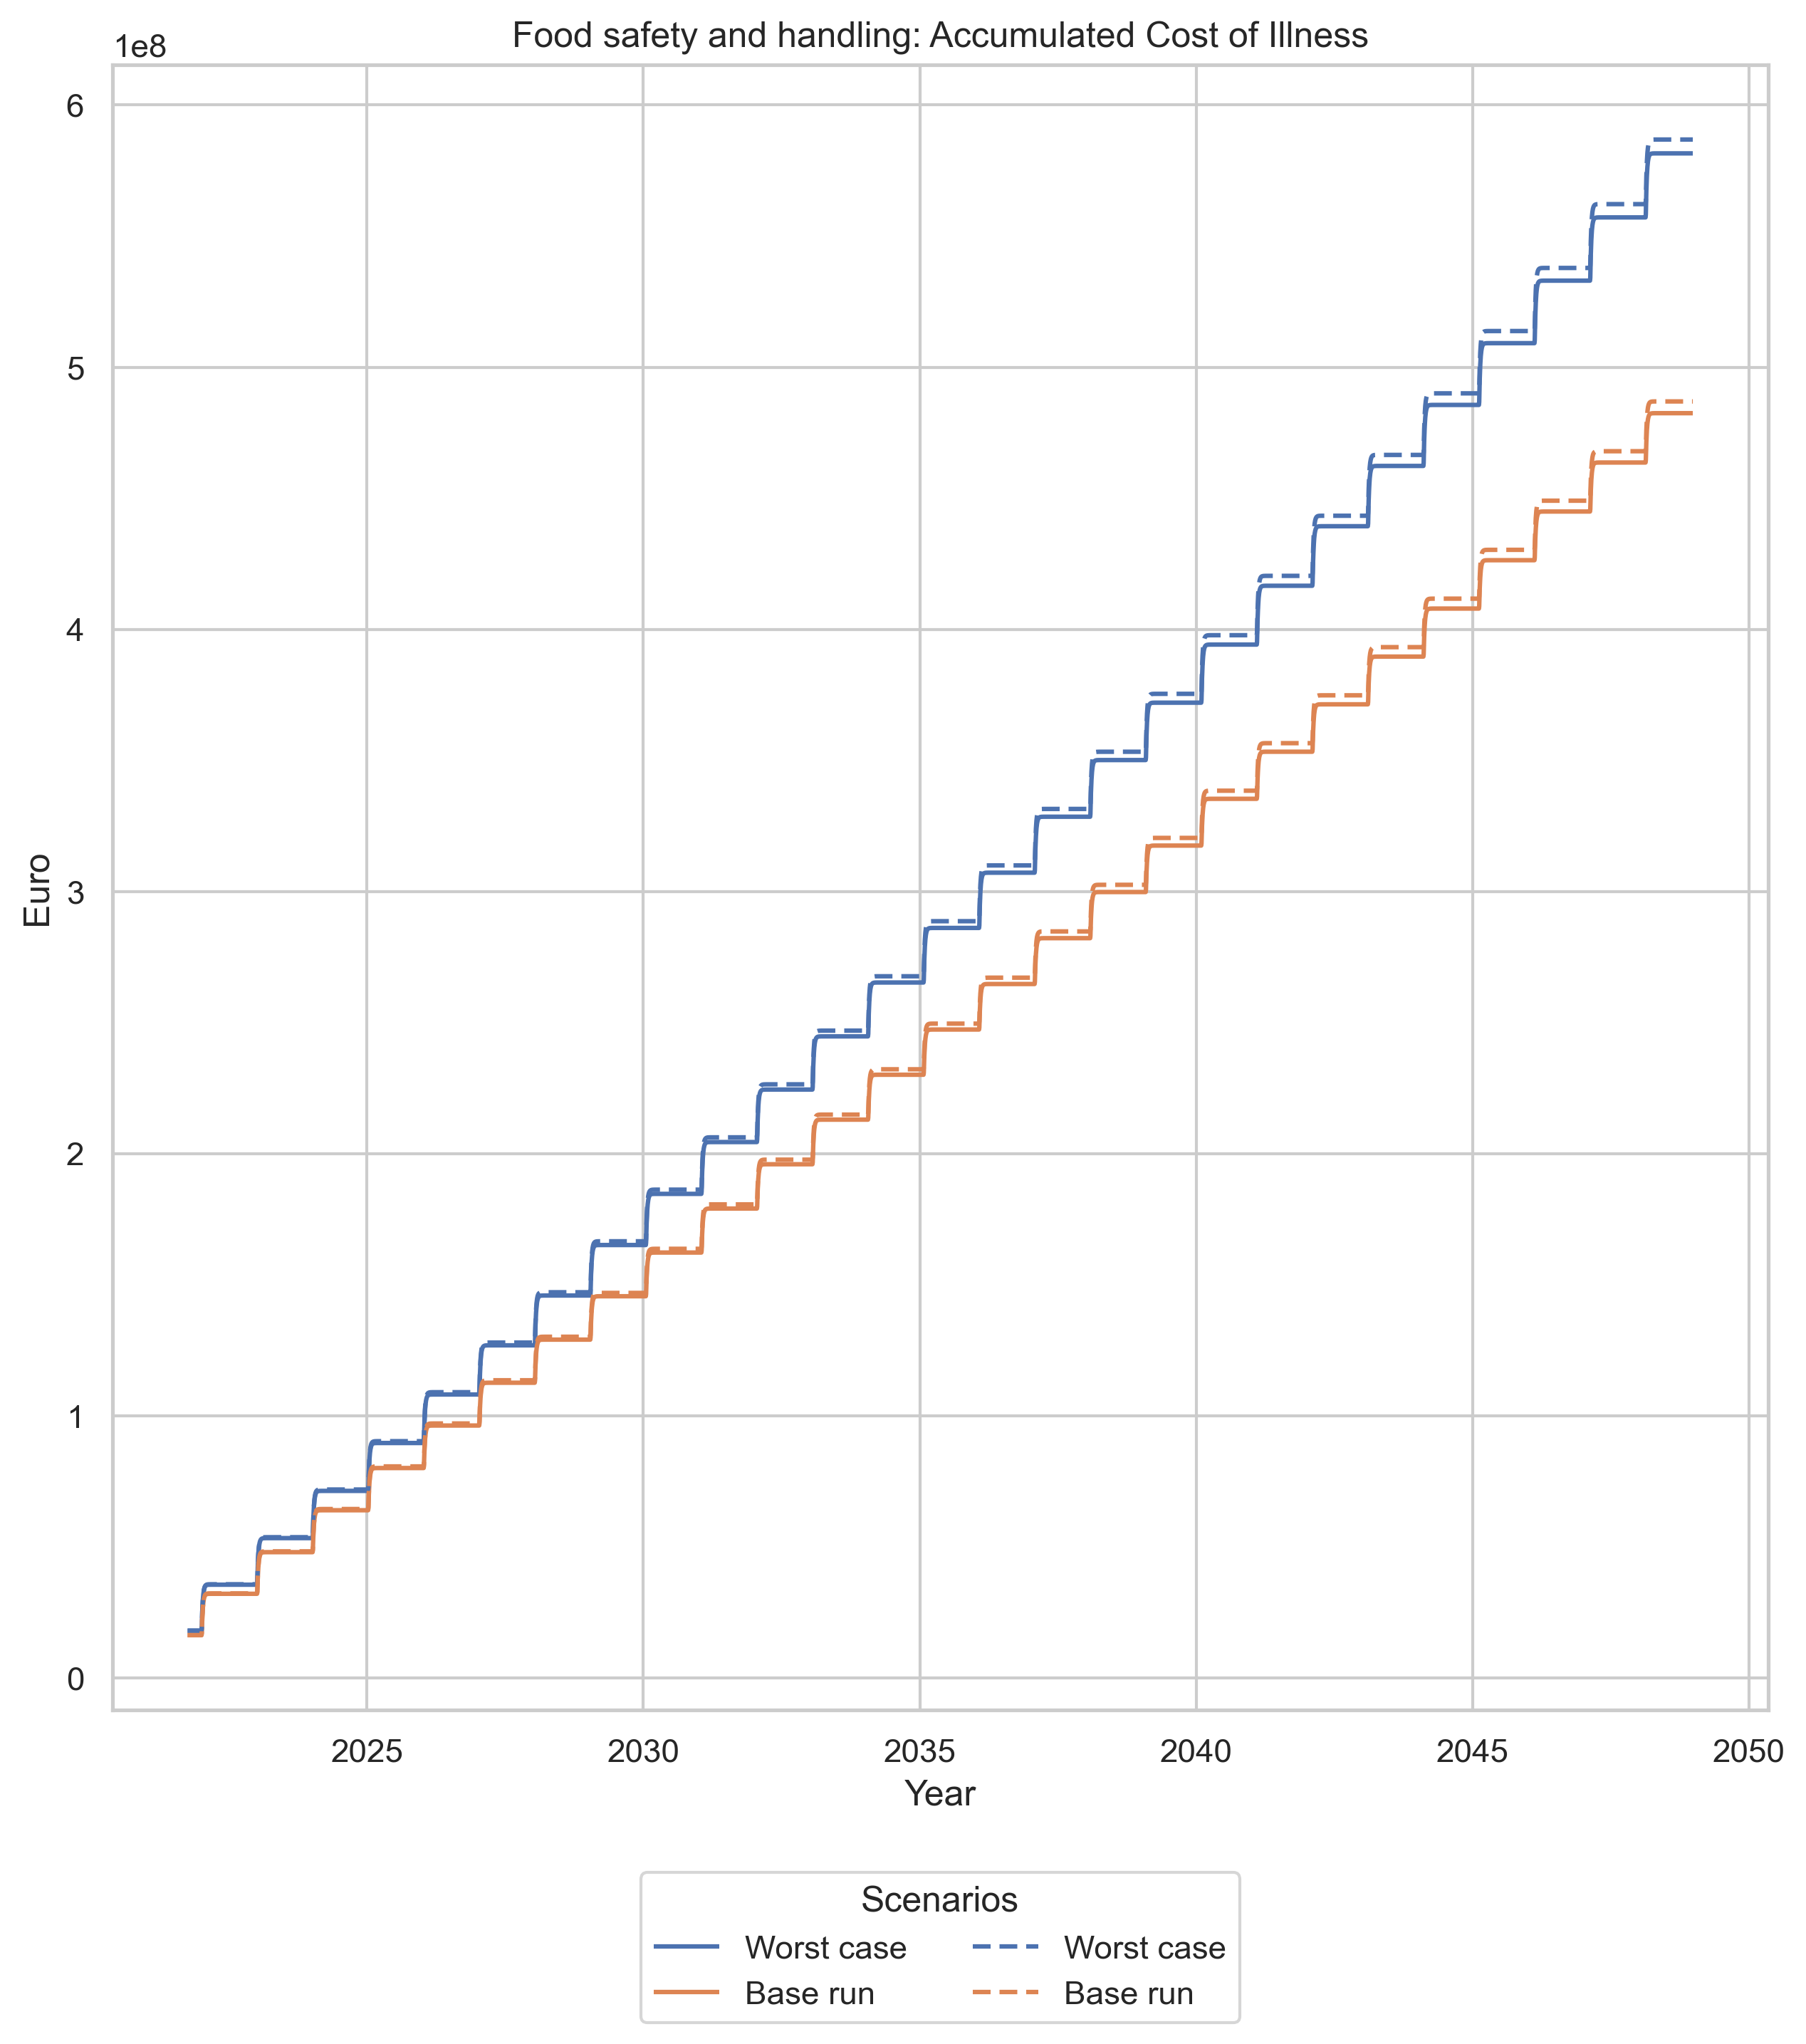
\includegraphics[width=1\textwidth]{images/fs_Base and Worst Case_acoi.png} 
        \caption{Accumulative cost of illness under the base and worst case scenarios, solid lines represent conditions with policy, dashed lines are condition without policy}
        \label{fig:fs_bwc_acoi}
    \end{minipage}
\end{figure}

However, this policy is considerably less effective and robust against environmental transmission, (rate of human infections/chicken infections from environment) where the policy has limited  (or no) effects under all scenarios.

As for the safe slaughtering policy, this policy has only a modest cost effectiveness (fs base and worst case acoi) achieved over the long term.


\subsubsection{Poultry consumption behaviour}
\label{sec: consumption behaviour}

This policy only activates under the worst case scenario. Essentially, this policy represents a last resort for the government. It's assumed that the government will not enact this policy except for under extenuating circumstances, whereby case numbers get so high that all other policy options are exhausted, and the government needs to ask citizens to reduce poultry consumption.

\begin{figure}[h!]
    \centering
    \begin{minipage}{0.45\textwidth}
        \centering
        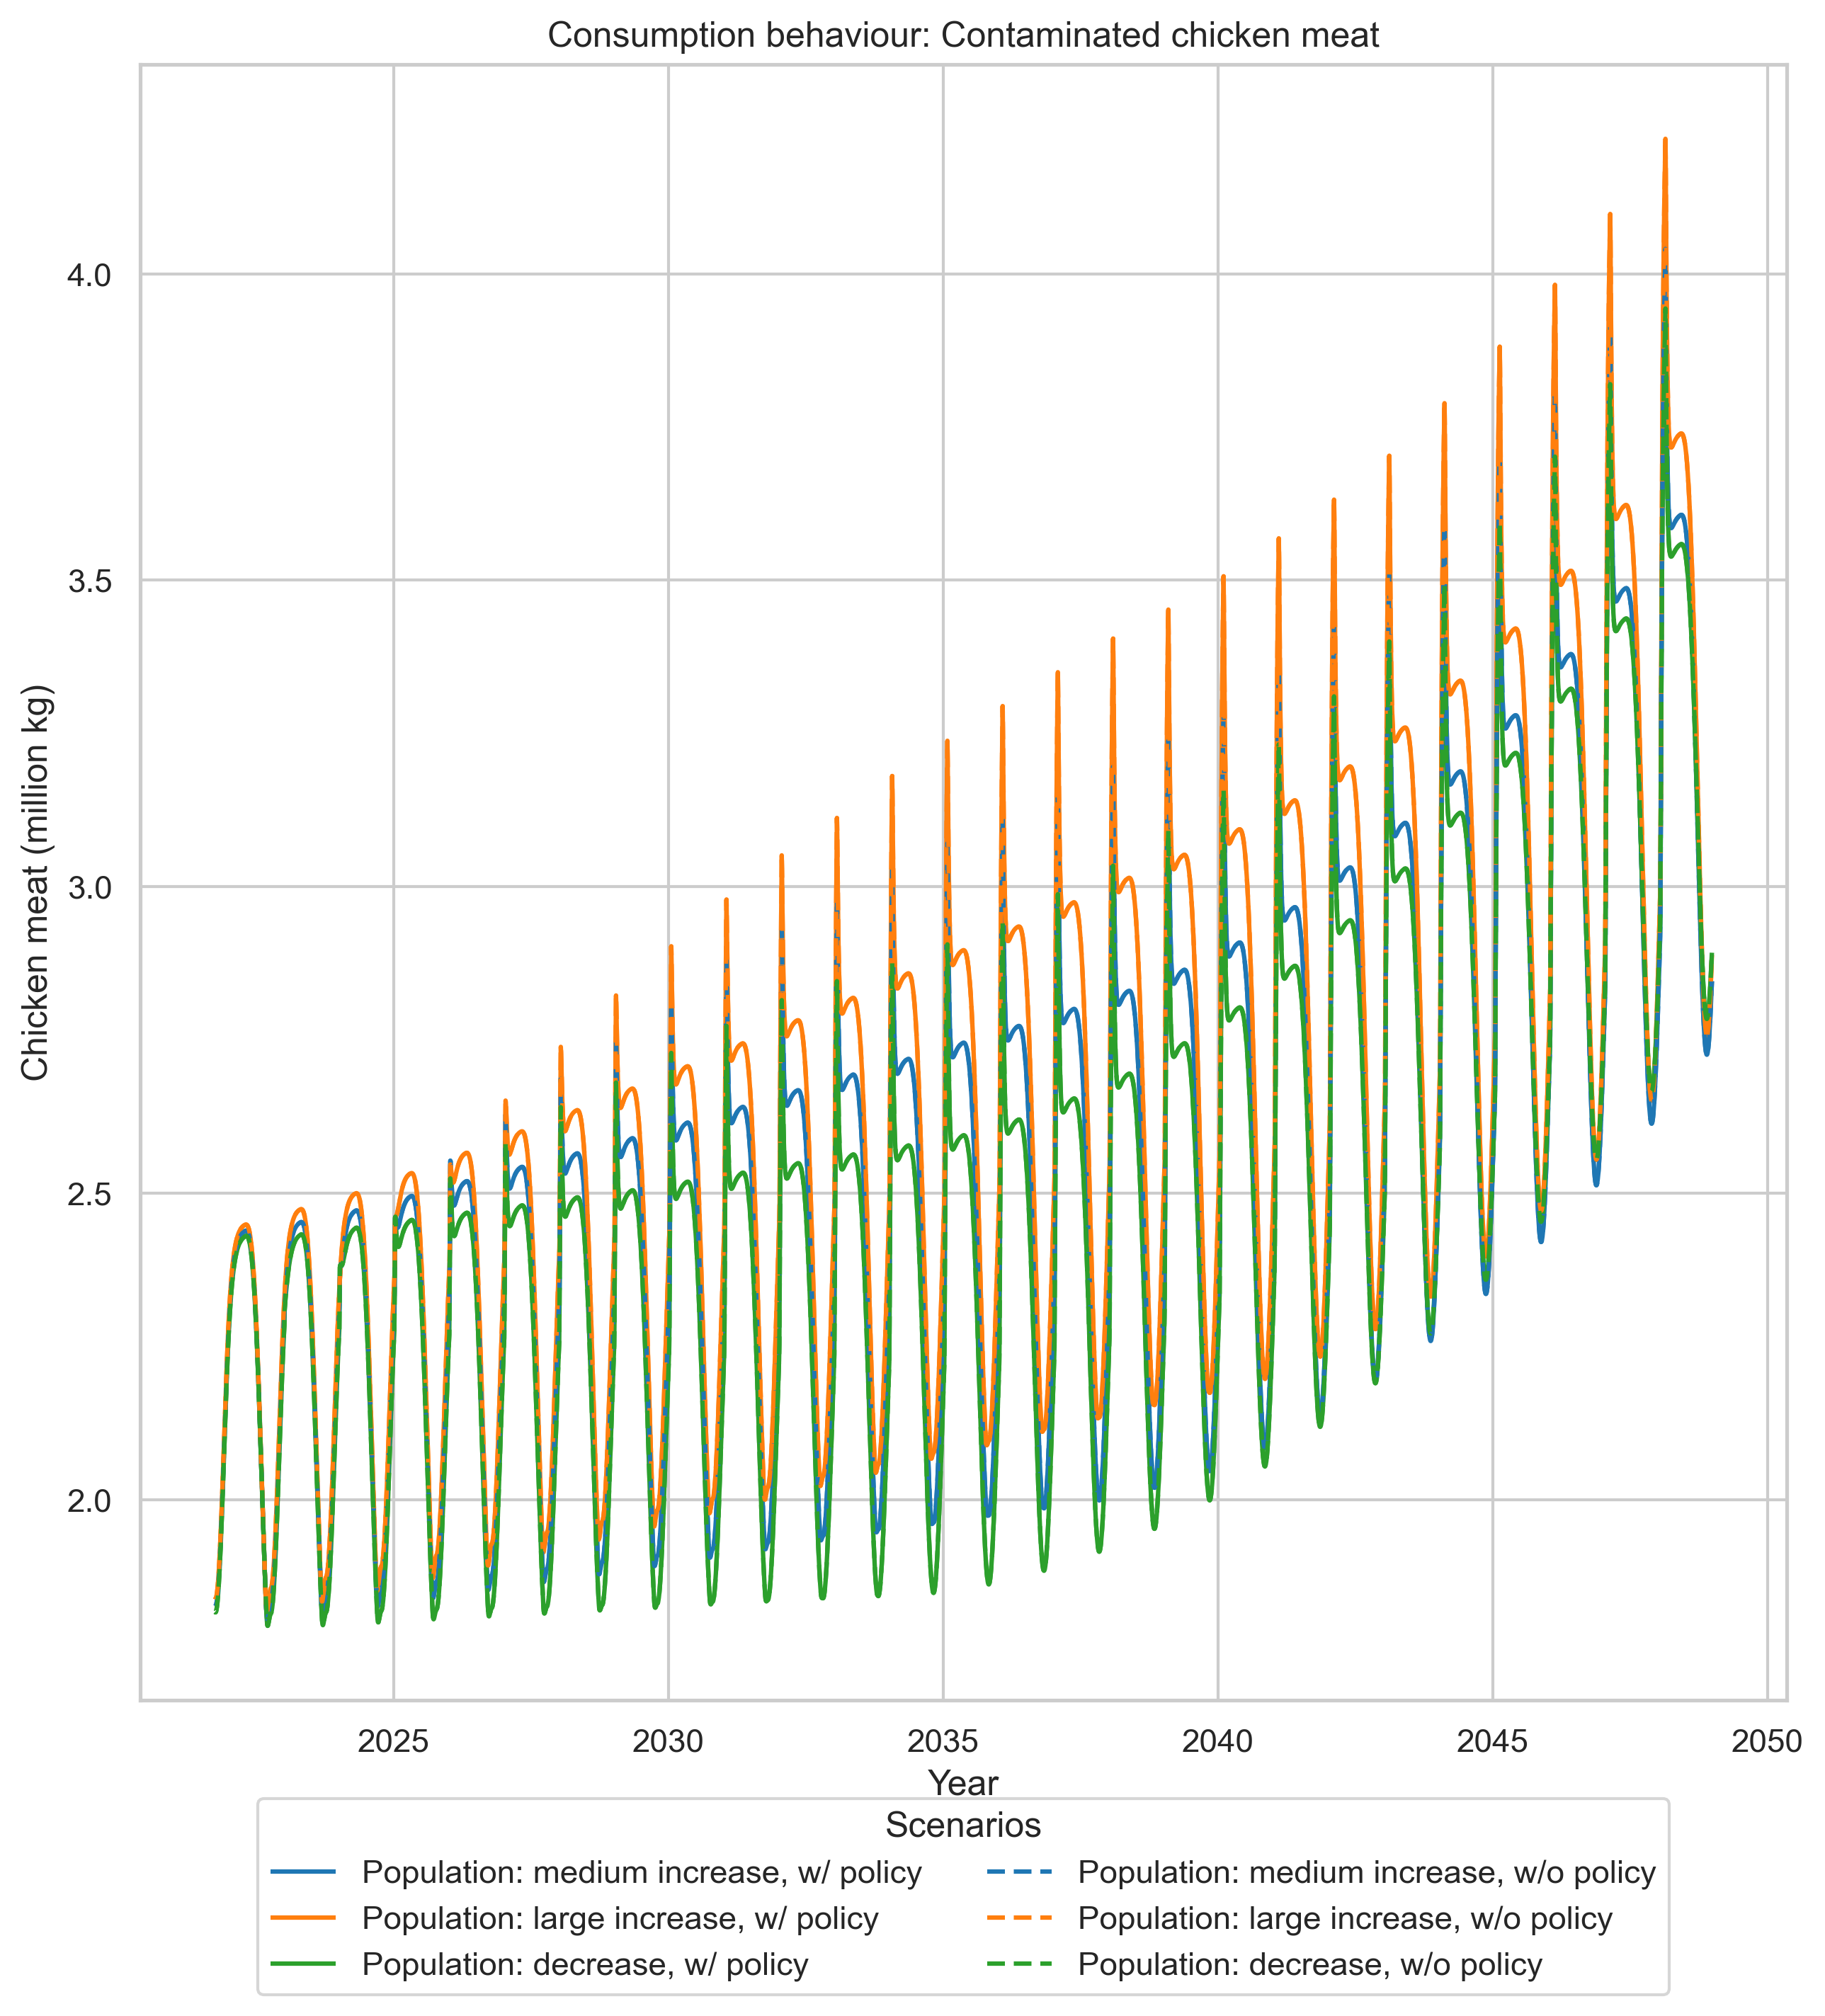
\includegraphics[width=1\textwidth]{images/cb_Population_meat.png}
        \caption{Contaminated chicken meat under different population scenarios, solid lines represent conditions with policy, dashed lines are condition without policy}
        \label{fig:pc_pop_meat}
    \end{minipage}\hfill
    \begin{minipage}{0.45\textwidth}
        \centering
        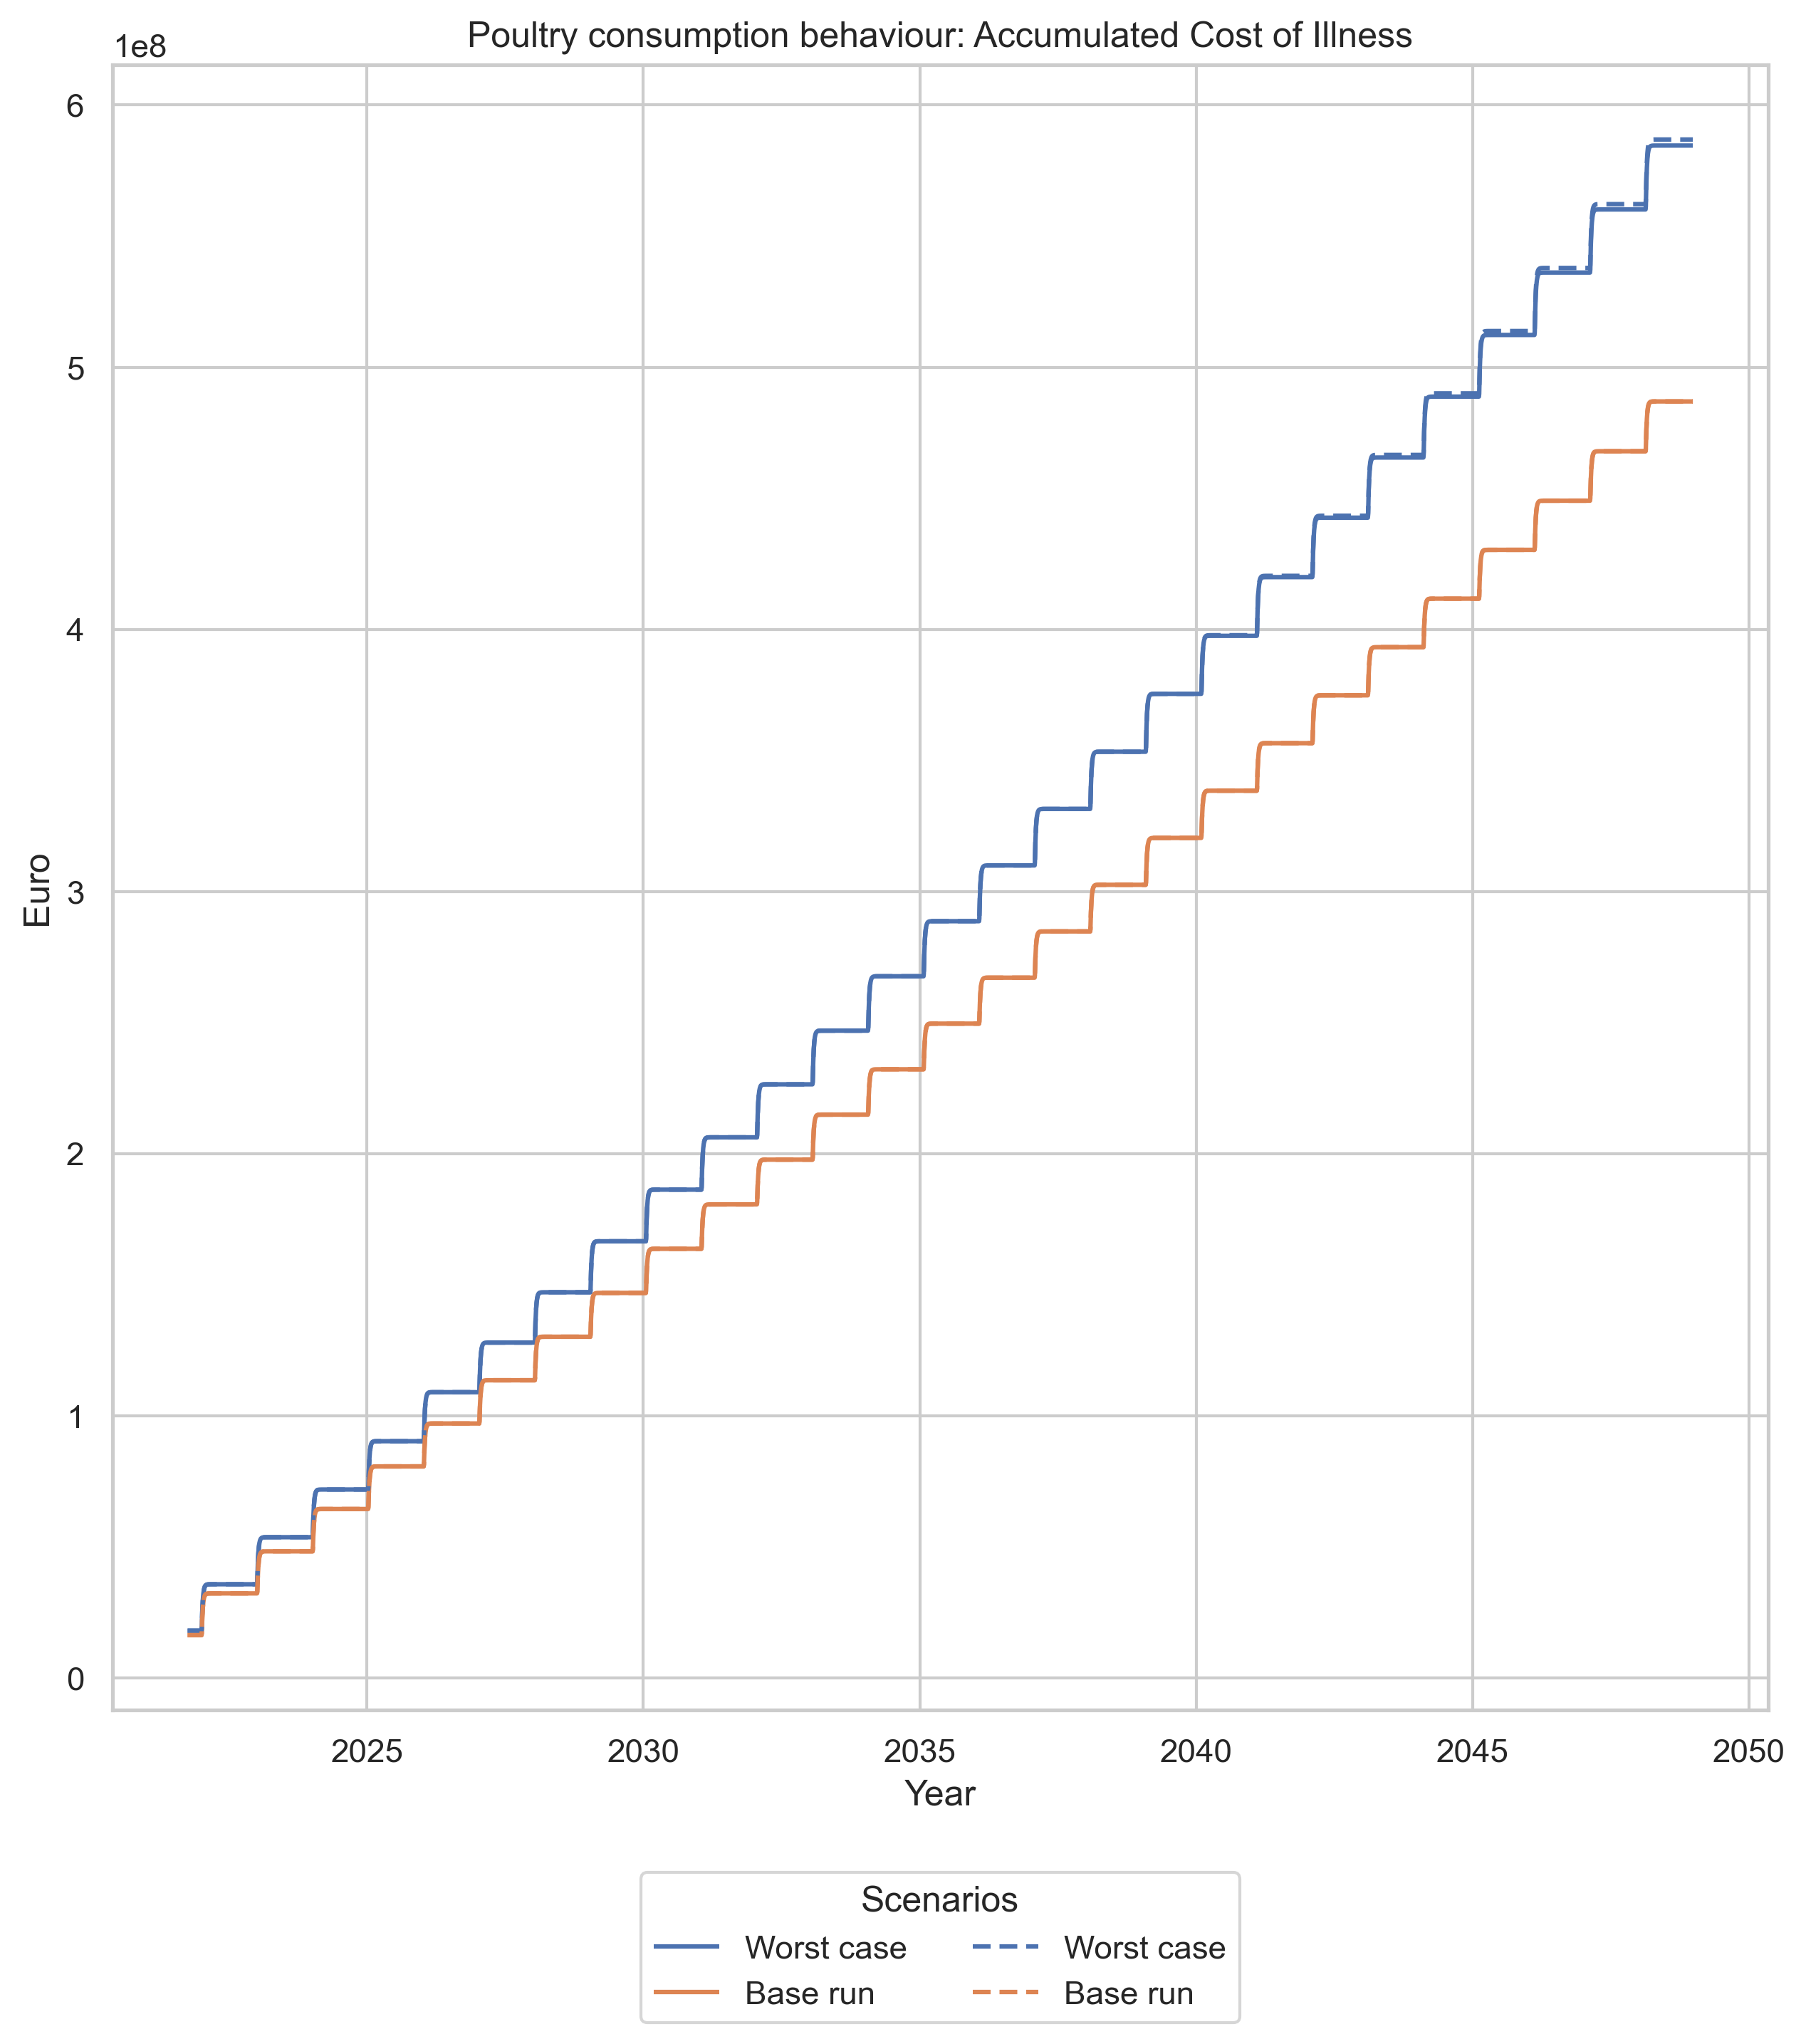
\includegraphics[width=1\textwidth]{images/cb_Base and Worst Case_acoi.png}
        \caption{Accumulative cost of illness under the base and worst case scenarios, solid lines represent conditions with policy, dashed lines are condition without policy}
        \label{fig:pc_bwc_acoi}
    \end{minipage}
\end{figure}

What can be seen is that when the policy is enacted, the amount of contaminated chicken meat decreases drastically. After some time, it even shows behaviour that is more desirable than without the policy enacted. However, the financial benefits of the policy aren't significant for quite a while, meaning that the savings for the government are minimal over the course of multiple years.

It is worth noting that this policy has an overlap with the consumption behavior that is already embedded in the model, that is, people might reduce their consumption on their own regardless of what government recommends, so the value added from this policy compared to the voluntary consumption reduction is even smaller.

\subsubsection{Reducing human exposure to flies}
\label{reducing human exposure to flies}
Reducing human exposure to flies was found to be the most robust of all the policies examined. It is also the second most cost-effective of the policies examined, in terms of reducing cost of illness. This is evident in (figure ec acoi worst best). This policy is effective for reducing the human-related KPIs (Cost of Illness, DALYs, Human Environmental Infections) across all scenarios. 

\begin{figure}[h!]
    \centering
    \begin{minipage}{0.45\textwidth}
        \centering
        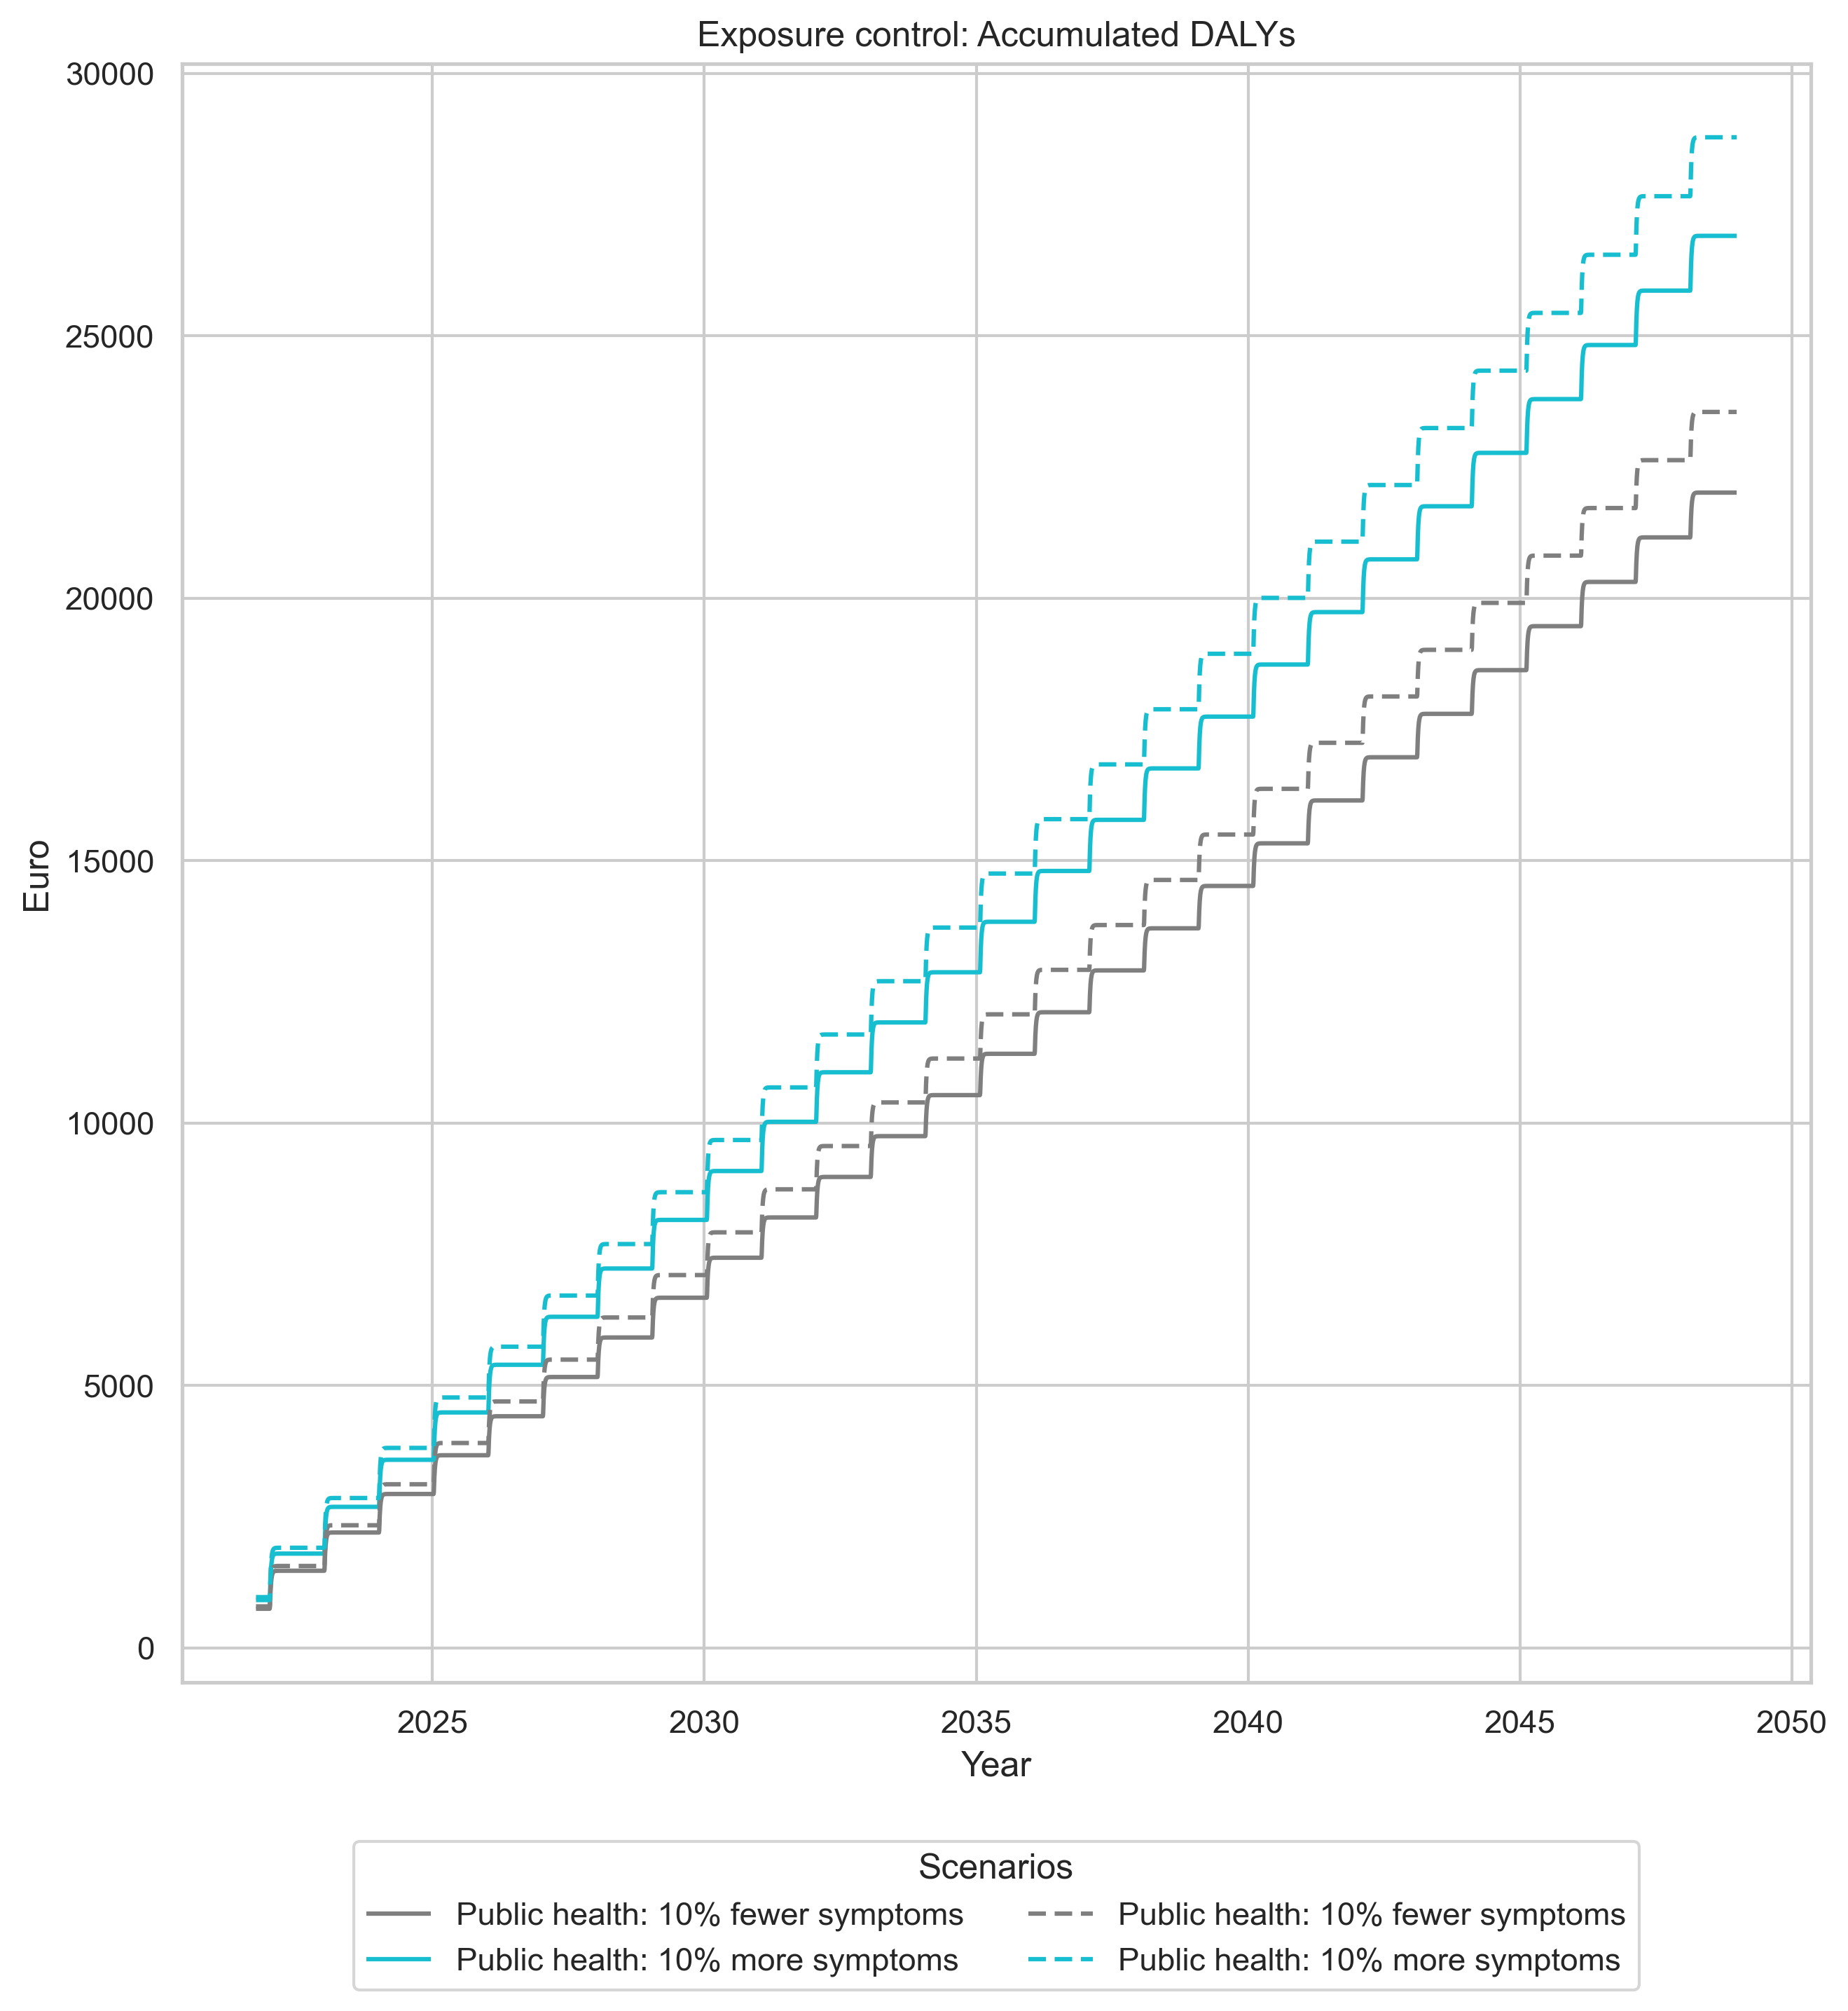
\includegraphics[width=1\textwidth]{images/ec_Public health_adaly.png}
        \caption{Accumulated DALYs under different public health scenarios, solid lines represent conditions with policy, dashed lines are condition without policy}
        \label{fig:ec_public_daly}
    \end{minipage}\hfill
    \begin{minipage}{0.45\textwidth}
        \centering
        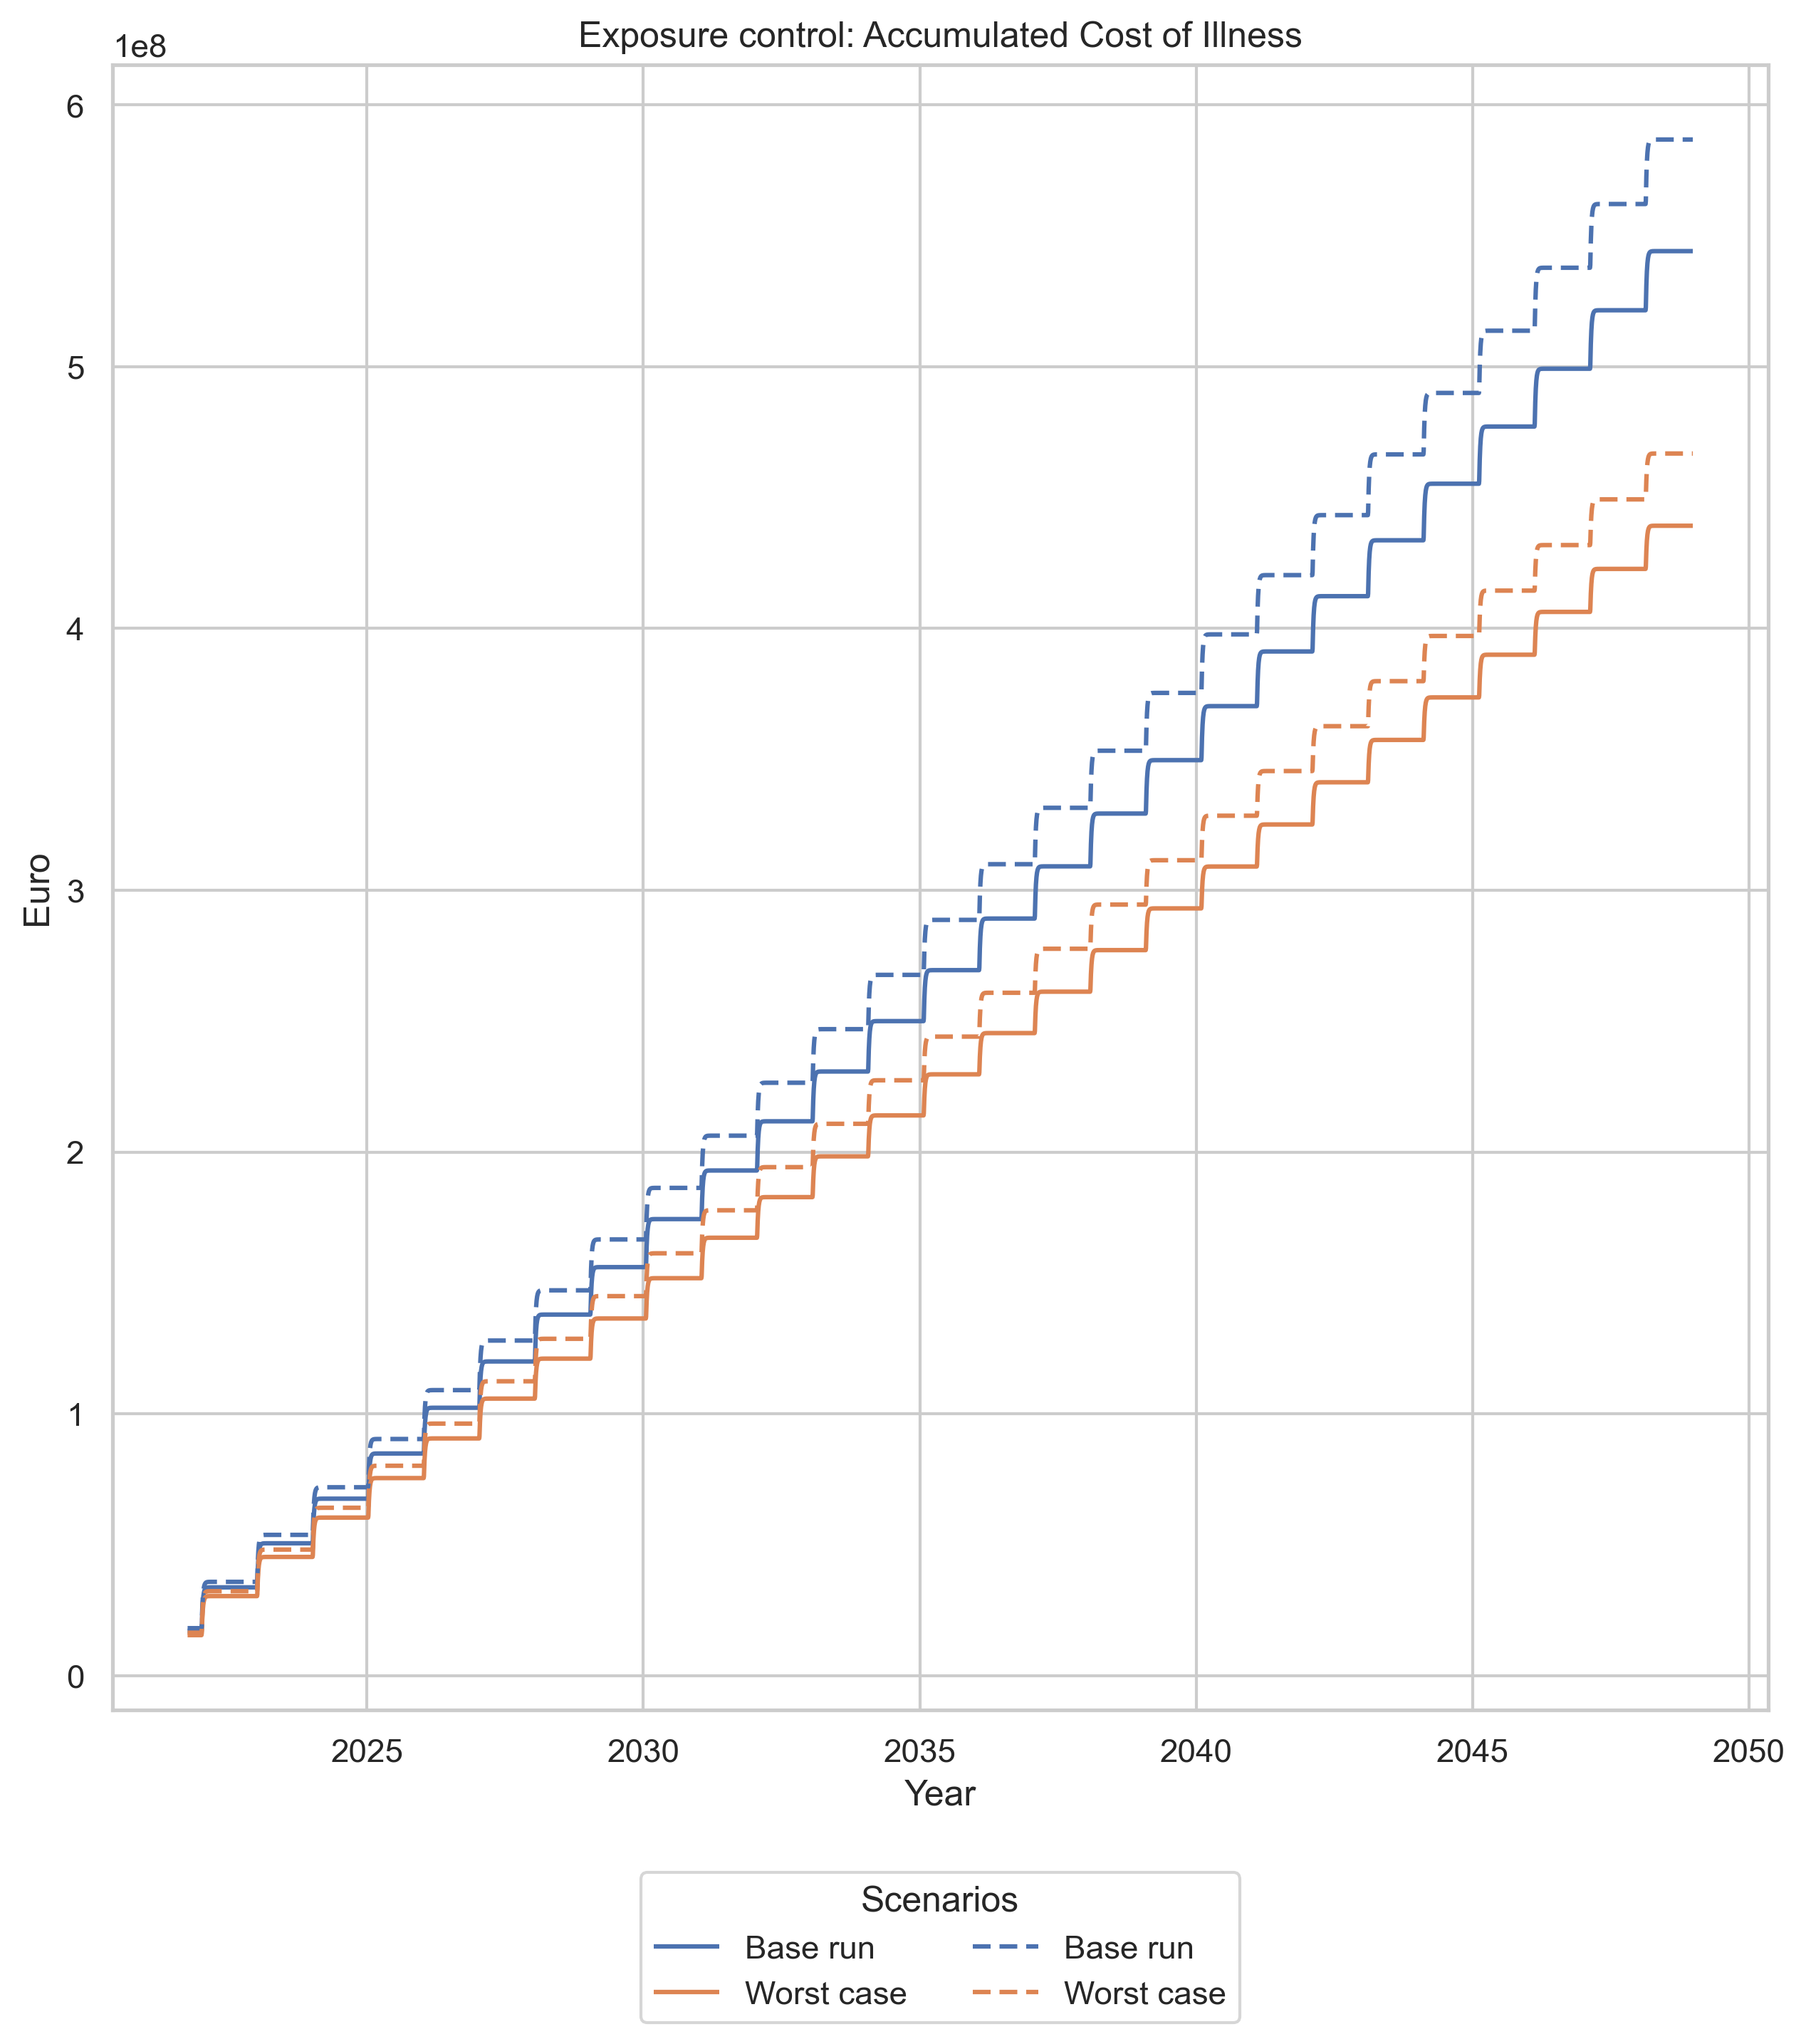
\includegraphics[width=1\textwidth]{images/ec_Base and Worst Case_acoi.png} 
        \caption{Accumulative cost of illness under the base and worst case scenarios, solid lines represent conditions with policy, dashed lines are condition without policy}
        \label{fig:ec_bwc_acoi}
    \end{minipage}
\end{figure}

It's believed that this policy is effective as it is a quick and direct means of reducing environmental infection, which subsequently reduces downstream KPIs. It doesn't require change in inelastic behaviour and doesn't replicate an existing behavioural uncertainty (like for changing consumption behaviour) so effects on infections can be observed relatively rapidly.

Given the cost-effectiveness and robustness of this policy, we would recommend that this policy be employed by the Dutch government to reduce human infection from environmental sources. We also recommend that further investigation into this policy be performed to ensure that it is representative of reality (for instance, by incorporating additional pathways for environmental transmission to occur). This may ultimately reduce the effectiveness of the policy, but would generate a more realistic picture for decision-makers.

